%%%%%%%%%%%%%%%%%%%%%%%%%%%%%%%%%%%%%%%%%%%%%%%%%%%%%%%%%%%%%%%%%%%%%%%%%%%%%%%%
%2345678901234567890123456789012345678901234567890123456789012345678901234567890
%        1         2         3         4         5         6         7         8

\documentclass[letterpaper, 10 pt, conference]{ieeeconf}  % Comment this line out if you need a4paper

%\documentclass[a4paper, 10pt, conference]{ieeeconf}      % Use this line for a4 paper

\IEEEoverridecommandlockouts                              % This command is only needed if you want to use the \thanks command

\overrideIEEEmargins                                      % Needed to meet printer requirements.

%In case you encounter the following error:
%Error 1010 The PDF file may be corrupt (unable to open PDF file) OR
%Error 1000 An error occurred while parsing a contents stream. Unable to analyze the PDF file.
%This is a known problem with pdfLaTeX conversion filter. The file cannot be opened with acrobat reader
%Please use one of the alternatives below to circumvent this error by uncommenting one or the other
%\pdfobjcompresslevel=0
%\pdfminorversion=4

% See the \addtolength command later in the file to balance the column lengths
% on the last page of the document

\usepackage{graphicx}  
% \usepackage{subcaption}
% \usepackage[caption=false,font=footnotesize]{subfig}
\usepackage{xcolor}
\usepackage{amsmath, amssymb}
\usepackage{mathtools}
\usepackage{algorithm}
\usepackage[noend]{algpseudocode}

\title{\LARGE \bf
Online Control Synthesis for Hyperproperties via Control Barrier Functions
}

\author{Georgios Mitsos$^{\star}$ and Siyuan Liu$^{\star}$% <-this % stops a space
\thanks{$^{\star}$ Department of Electrical Engineering, Eindhoven University of Technology, 5612 AE Eindhoven, The Netherlands {\tt\small \{g.mitsos, s.liu5\} @tue.nl}}%
}

% Algorithms 
\newcommand{\algorithmautorefname}{Algorithm}
\algrenewcommand{\Require}{\Statex \textbf{Input:}}  
\algrenewcommand{\Ensure}{\Statex \textbf{Output:}} 

% New environments with autoref support
\newtheorem{remark}{Remark}
\newtheorem{definition}{Definition}
\newtheorem{theorem}{Theorem}
\newtheorem{lemma}{Lemma}
\newtheorem{proposition}{Proposition}
\newtheorem{problem}{Problem}
\newtheorem{assumption}{Assumption}

\begin{document}

\maketitle
\thispagestyle{empty}
\pagestyle{empty}


%%%%%%%%%%%%%%%%%%%%%%%%%%%%%%%%%%%%%%%%%%%%%%%%%%%%%%%%%%%%%%%%%%%%%%%%%%%%%%%%
\begin{abstract}
    Complex tasks are commonly specified using formal languages such as linear temporal logic and signal temporal logic, which express specifications over a single execution of a system. In contrast, hyperproperties capture requirements that relate multiple executions and allow universal ($\forall$) and existential ($\exists$) quantification over traces. Most hyperproperties of interest can be expressed using alternating quantifier structures of the form $\exists \, \forall$ and $\forall \, \exists$. The former requires the existence of a single reference trajectory that satisfies a given relation with all executions, while the latter requires that for every execution there exists a corresponding trajectory satisfying the relation. Representative examples include initial-state robustness and opacity, respectively. Initial-state robustness requires that trajectories arising from uncertainty in the initial condition remain close to a reference execution, whereas opacity requires that every secret execution be observationally indistinguishable from some non-secret execution.
    In this work, we develop two online control synthesis frameworks for continuous-time input-affine systems that enforce such hyperproperties with formal guarantees. Our approach translates hyperproperty specifications into forward-invariance conditions via self-composition of the system and control barrier functions defined on the augmented system. The resulting constraints are enforced online through quadratic programs that minimally modify a nominal controller and are solved in a sampled-data fashion. The proposed methods are illustrated through two case studies.
\end{abstract}


%%%%%%%%%%%%%%%%%%%%%%%%%%%%%%%%%%%%%%%%%%%%%%%%%%%%%%%%%%%%%%%%%%%%%%%%%%%%%%%%
\section{Introduction}

Autonomous cyber-physical systems (CPS) increasingly operate in open environments where correct behavior must be ensured not only along a single closed-loop trajectory, but also across families of trajectories arising from uncertainty and adversarial observation. At the same time, modern robotic systems must accomplish increasingly complex tasks while providing formal correctness guarantees. Formal specification and synthesis methods based on temporal logics have therefore become central tools for motion planning and control \cite{fainekos2009, kloetzer2008}, enabling the expression of rich, high-level tasks beyond classical reach--avoid objectives \cite{lavalle2006, karaman2011} and supporting fully-automated and correct-by-design controller synthesis for broad system classes \cite{smith2011}.

A fundamental limitation, however, is that standard temporal logics specify requirements over individual executions. Many practically important requirements in robotics and CPS are inherently relational, that is, they quantify how multiple executions compare \cite{wang2020}. Examples include \emph{robustness to initial-state uncertainty}, requiring that all trajectories starting in a prescribed uncertainty set should stay close to a nominal execution or converge to it, and information-flow security properties \cite{zhao2024} such as \emph{opacity} \cite{lafortune2018}, requiring that an external observer should be unable to infer whether the system has executed a secret behavior. Such multi-execution requirements, in general, cannot be expressed in classic temporal logics, leading to the introduction of hyperproperties in \cite{clarkson2010}. Hyperlogics such as HyperLTL and HyperCTL extend these with explicit quantification over multiple traces \cite{clarkson2014}, enabling formulas with alternating universal ($\forall$) and existential ($\exists$) quantifiers \cite{finkbeiner2015}. For real-valued trajectories and continuous-space CPS, HyperSTL extends signal temporal logic with trace quantifiers to express hyperproperties over real-valued signals \cite{nguyen2017}.

Verification of hyperproperties has advanced substantially via automata-theoretic model checking \cite{clarkson2014}, dedicated tools \cite{finkbeiner2015}, and, more recently, certificate-based approaches for discrete-time dynamical systems \cite{anand2024}. In contrast, controller synthesis for hyperproperties remains comparatively less explored. In both cases, most of the existing methods target finite-state models \cite{wang2020, finkbeiner2015} or discrete-time systems \cite{anand2024, zhao2025}, leaving continuous-time largely unexplored. Moreover, CPS often require online, real-time control capable of reacting react to disturbances and uncertainty during operation. Current hyperproperty-based control synthesis methods, however, are predominantly offline. A similar limitation arises in opacity-preserving control synthesis, where existing approaches are primarily developed for discrete-event systems (DES) \cite{yang2023, yu2022} or for discrete-time systems with offline synthesis \cite{zhong2025}. 

In parallel, a growing body of work in robotics employs control barrier functions (CBFs)  provide an optimization-based framework for online synthesis of safety-critical controllers by rendering a specified safe set forward invariant \cite{ames2014, ames2019}. Moreover, CBF-based methods have been integrated with temporal-logic objectives to enable real-time control for complex tasks \cite{srinivasan2021, lindemann2019}. Robustness extensions of CBFs address input disturbances and model perturbations by guaranteeing invariance of larger safe sets \cite{xu2015, kolathaya2019}. However, these approaches do not address uncertainty in the initial condition.

Moreover, in many task-planning approaches the executions associated by universal quantifiers are not generated by the synthesized controller, but instead they range over all admissible system behaviors \cite{wang2020, zhao2025}. As a result, the controller must satisfy the specification against every possible behavior of the universally quantified traces, effectively reduces the problem to verification. From a control perspective, however, executions are generated by an initial state and a control input sequence. Consider a $\forall \, \exists$ hyperproperty requiring that for every execution there exists another execution satisfying a relational condition $\varphi$: $\forall \pi \, \exists \pi'. \varphi(\pi, \pi')$, where $\pi$ and $\pi'$ denote system executions. Since executions arise from initial states and control inputs, i.e., $\pi = \pi(\mathbf{x}_0, \mathbf{u})$, this requirement can eqivalently be expressed as $\forall \mathbf{x}_0 \, \exists \mathbf{x}_0' \, \exists u \, \exists u'.  \varphi(\pi, \pi')$, where $\mathbf{x}_0$, $\mathbf{x}_0'$ are initial states, and $u$, $u'$ are the control inputs generating $\pi$ and $\pi'$.

This paper bridges hyperproperty specifications and online CBF-based control for continuous-time control-affine systems. \textcolor{red}{motivate contraction: nominal trajectory satisfies tasks, and initial conditions are "forgotten"} We first consider robustness hyperproperties capturing initial-state uncertainty of the form (i) $\exists \pi \, \forall \pi'.\, \mathbf{G}\big(\|\pi - \pi'\|\leq \delta\big)$ and (ii)
$\exists \pi \, \forall \pi'.\, \mathbf{F}\big(\|\pi - \pi'\|\leq \varepsilon\big)$where $\mathbf{G}$ and $\mathbf{F}$ denote the temporal operators \emph{always} and \emph{eventually}, respectively. Here, $\pi$ is a nominal execution and $\pi'$ ranges over executions originating from an uncertainty set around the nominal initial state. The former requires all executions to remain within a $\delta$-neighborhood of the nominal trajectory, while the latter requires eventual contraction within an $\varepsilon$-neighborhood. We then cosider information-flow security hyperproperties and focus on opacity, naturally expressed as a $\forall \, \exists$ hyperproperty requiring that every secret system behavior admits a non-secret behavior producing an indistinguishable observation to an intruder equipped with an observation model. Using a notion of approximate opacity \cite{yin2021} suitable for metric outputs and continuous-time systems, we construct CBF conditions on a self-composed (two-trace) system so that opacity can be enforced as a forward-invariance condition. The resulting constraints are implemented online via a CBF-based quadratic program (QP). The proposed framework enables hyperproperty satisfaction in real time and can be combined with CBFs derived from temporal-logic specifications \cite{srinivasan2021, lindemann2019} within the same QP. Theoretical guarantees and illustrative case studies demonstrate the approach.

%%%%%%%%%%%%%%%%%%%%%%%%%%%%%%%%%%%%%%%%%%%%%%%%%%%%%%%%%%%%%%%%%%%%%%%%%%%%%%%%
\section{Preliminaries}

\textbf{Notation.} Let $\mathbb{R}$, $\mathbb{Z}$, and $\mathbb{N}$ denote the sets of real numbers, integers and positive integers, respectively, and let $\mathbb{R}_{\ge 0}$ denote the set of nonnegative real numbers. For any $n, m \in \mathbb{N}$, $\mathbb{R}^n$ denotes the space of $n$-dimensional column vectors and $\mathbb{R}^{n \times m}$ the space of $n \times m$ real matrices. Vectors are denoted by bold lowercase letters and matrices by bold uppercase letters. The vectors of all zeros and all ones are denoted by $\mathbf{0}$ and $\mathbf{1}$, respectively. For any $\mathbf{x} = \begin{bmatrix} x_1 & \dots & x_n \end{bmatrix}^\top \in \mathbb{R}^n$, $\|\mathbf{x}\|$ denotes the Euclidean norm, i.e., $\|\mathbf{x}\| = \sqrt{\mathbf{x}^\top \mathbf{x}}$, and $\|\mathbf{x}\|_\infty$ denotes the infinity norm, i.e., $\|\mathbf{x}\|_\infty = \max_i{|x_i|}$. The notation $\operatorname{diag}(\lambda_1, \lambda_2, \dots)$ denotes the diagonal matrix with entries $\lambda_1$, $\lambda_2$, $\dots$. A continuous function $\alpha: \mathbb{R}_{\ge 0} \to \mathbb{R}_{\ge 0}$ is of class-$\mathcal{K}$ if it is strictly increasing, and with $\alpha(0) = 0$. A function $\beta: \mathbb{R}_{\ge 0} \times \mathbb{R}_{\ge 0} \to \mathbb{R}_{\ge 0}$ is of class-$\mathcal{K} \mathcal{L}$ if (i) for each fixed $s$, $\alpha(r, s)$ is class-$\mathcal{K}$, and (ii) for each fixed $r$, $\alpha(r, s)$ is decreasing in $s$ and with $\lim_{s \to \infty} \alpha(r, s) = 0$. Given a continuously differentiable function $V : \mathbb{R}^n \to \mathbb{R}$ and a vector field $\mathbf{f} : \mathbb{R}^n \to \mathbb{R}^n$, the Lie derivative of $V$ along $\mathbf{f}$ is defined as $L_\mathbf{f} V(\mathbf{x}) = \tfrac{\partial V}{\partial \mathbf{x}} \mathbf{f}(\mathbf{x})$.

\subsection{System model}

We consider a nonlinear input-affine control system
\begin{equation} \label{eq:system}
    S =
    \Bigg\{
    \begin{aligned}
        &\dot{\mathbf{x}}(t) = \mathbf{f}(\mathbf{x}(t)) + \mathbf{g}(\mathbf{x}(t)) \, \mathbf{u}(t), \quad \mathbf{x}(0) = \mathbf{x}_0\\
        &y(t) = h(\mathbf{x}(t)),
    \end{aligned}
    \Bigg.
\end{equation}
where $\mathbf{x} \in \mathbb{X} \subseteq \mathbb{R}^n$ denotes the state, $\mathbf{u} \in \mathbb{U} \subset \mathbb{R}^m$ the control input, and $y \in \mathbb{Y} \subseteq \mathbb{R}^p$ the output. The initial state $\mathbf{x}_0$ belongs to $\mathbb{X}_0 \subseteq \mathbb{X} \subset \mathbb{R}^n$. The functions $\mathbf{f}: \mathbb{R}^n \rightarrow \mathbb{R}^n$ and $\mathbf{g}: \mathbb{R}^n \rightarrow \mathbb{R}^{n \times m}$ are locally Lipschitz continuous, and $\mathbf{h}: \mathbb{R}^n \rightarrow \mathbb{R}^p$ is continuously differentiable.

Given a controller $\boldsymbol{\nu}(t): \mathbb{R}_{\ge 0} \rightarrow \mathbb{U}$ and an initial state $\mathbf{x}_0 \in \mathbb{X}_0$, we denote by $\mathbf{x}_{\mathbf{x}_0, \boldsymbol{\nu}}(t): \mathbb{R}_{\ge 0} \to \mathbb{X}$ the corresponding closed-loop trajectory.

\subsection{Control Lyapunov functions}

Control Lyapunov functions (CLFs) \cite{sontag1983,artstein1983}
provide a constructive tool for stabilizing nonlinear control systems as in \eqref{eq:system}. The idea is to design a feedback controller that drives
a positive definite function $V$ to zero along system trajectories.

\begin{definition}
A continuously differentiable positive definite function $V:\mathbb{R}^n \rightarrow \mathbb{R}_{\ge 0}$ is a CLF for the system \eqref{eq:system} with respect to the point $\mathbf{x}^\star = \mathbf{0}$ there exists a locally Lipschitz class-$\mathcal{K}$ function $\alpha$ such that, for all $\mathbf{x} \neq \mathbf{0}$,
\begin{equation} \label{eq:clf}
    \inf_{\mathbf{u}\in\mathbb{U}} \left[ \Big( \frac{\partial V}{\partial \mathbf{x}}(\mathbf{x}) \Big)^\top \! \left(\mathbf{f}(\mathbf{x}) + \mathbf{g}(\mathbf{x}) \, \mathbf{u} \right) \right] \le -\alpha(V(\mathbf{x})).
\end{equation}
\end{definition}

\begin{theorem} \label{thm:stability}
    \cite{artstein1983} If $V$ is a CLF, then any continuous feedback controller $\mathbf{u}(\mathbf{x})$ such that $\big(\tfrac{\partial V}{\partial \mathbf{x}} (\mathbf{x}) \big)^\top \left(\mathbf{f}(\mathbf{x}) + \mathbf{g}(\mathbf{x}) \, \mathbf{u} \right) \le -\alpha(V(\mathbf{x}))$ renders the system \eqref{eq:system} globally asymptotically stable (GAS), i.e., $  \lim_{t \to \infty} \mathbf{x} = \mathbf{0}$.
\end{theorem}

If this holds, there exists a feedback controller $\mathbf{u}(\mathbf{x})$ that renders the equilibrium $\mathbf{x}^\star=\mathbf{0}$ asymptotically stable.

\subsection{Control barrier functions}

Consider a system as in \eqref{eq:system} and a set $\mathcal{C}$, which is defined as the superlevel set of a continuously differentiable function $b: \mathbb{R}^n \to \mathbb{R}$, i.e., 
\begin{equation} \label{eq:safe_set}
    \mathcal{C} = \{\mathbf{x} \in \mathbb{X} \mid b(\mathbf{x}) \ge 0 \}.
\end{equation}  

\begin{definition}\label{def:cbf}
Consider a set defined as in \eqref{eq:safe_set}. The function $b(\mathbf{x})$ is a CBF if there exists a locally Lipschitz class-$\mathcal{K}$ function $\alpha$ such that 
\begin{equation} \label{eq:cbf}
   \sup_{\mathbf{u} \in \mathbb{U}} \Big[ \Big(\frac{\partial b}{\partial \mathbf{x}}(\mathbf{x}) \Big)^\top (\mathbf{f}( \mathbf{x}) + \mathbf{g}( \mathbf{x}) \, \mathbf{u})\Big] \ge -\alpha(b(\mathbf{x})).
\end{equation}
\end{definition}

\begin{theorem} \label{thm:forward_invariance}
    \cite{ames2019} Let $\mathcal{C} \subset \mathbb{X}$ be defined as the superlevel set of a continuously differentiable function $b: \mathbb{R}^n \rightarrow \mathbb{R}$. If $b$ is a CBF, then any Lipschitz continuous controller $\mathbf{u}(\mathbf{x})$ such that $\big(\tfrac{\partial b}{\partial \mathbf{x}}(\mathbf{x}) \big)^\top \!(\mathbf{f}( \mathbf{x}) \!+\! \mathbf{g}( \mathbf{x}) \mathbf{u}) \!\ge\! -\alpha(b(\mathbf{x}))$ renders $\mathcal{C}$ forward invariant for the system \eqref{eq:system}, i.e., $  \mathbf{x}(0) \in \mathcal{C} \Rightarrow \mathbf{x}(t) \in \mathcal{C} $ for all $t \in \mathbb{R}_{\ge 0}$.
\end{theorem}

% \subsection{Safety}

% Safety is characterized as a forward invariance property of a designated safe set. Let $\mathcal{S} \subseteq \mathbb{X}$ be defined as the superlevel set of a continuously differentiable function $h: \mathbb{R}^n \to \mathbb{R}$, namely, $\mathcal{S} = \{\mathbf{x \in \mathbb{X}} \mid h(\mathbf{x})\ge 0 \}$. The boundary of $\mathcal{S}$ is denoted by 
% $\partial \mathcal{S} = \{ \mathbf{x} \in \mathbb{X} \mid h(\mathbf{x}) = 0 \}$. By Nagumo's theorem, the set $\mathcal{S}$ is forward invariant if and only if $\dot h(\mathbf{x}) \ge 0$ for all $\mathbf{x} \in \partial \mathcal{S}$. 

% The \emph{unsafe set} $\mathbb{X}_u$ is defined as the complement of $\mathcal{C}$. i.e., $\mathbb{X}_u = \mathbb{X} \setminus \mathcal{C}$. The safety control synthesis problem consists of designing a controller that renders the safe set $\mathcal{C}$ forward invariant for the closed-loop system.
% \begin{definition} \label{def:safety}
%     Consider a continuous-time control system as in \eqref{eq:system}, a controller $\boldsymbol{\nu}(t): \mathbb{R}_{\ge 0} \rightarrow \mathbb{U}$, and an initial state $\mathbf{x}_0 \in \mathbb{X}_0$. A trajectory $\mathbf{x}_{\mathbf{x}_0, \boldsymbol{\nu}}(t)$ is \emph{safe} if $\mathbf{x}_{\mathbf{x}_0, \boldsymbol{\nu}}(t) \notin \mathbb{X}_u$ for all $t \in \mathbb{R}_{\ge 0}$.
% \end{definition}

\subsection{Linear temporal logic}

Let $\mathcal{AP}$ be a finite set of atomic propositions. The syntax of LTL is defined recursively \cite{baier2008}:
\begin{equation*} \label{eq:ltl}
    \varphi \Coloneqq \pi \mid \lnot \, \varphi \mid \varphi_1 \land \varphi_2 \mid \varphi_1 \, \mathcal{U} \, \varphi_2,
\end{equation*}
where $\pi \in \mathcal{AP}$, and $\varphi$, $\varphi_1$, $\varphi_2$ are LTL formulas, and $\mathcal{U}$ denotes the \emph{until} operator. The disjunction ($\lor$) is derived as $\varphi_1 \lor \varphi_2 {:=} \lnot (\lnot \varphi_1 \land \lnot \varphi_2)$, the Boolean $true$ as $p \lor \lnot p$, while the temporal operators \emph{eventually} ($\lozenge$) and \emph{always} ($\square$) are defined as $\lozenge \varphi  {:=} true \ \mathcal{U} \ \varphi$, and $\square \, \varphi {:=} \lnot  \lozenge \, \lnot \varphi$, respectively. The $\emph{next}$ ($\mathcal{X}$) operator is omitted since it is not meaningful for continuous-time systems.

A trace is an infinite word $\sigma = \sigma_0 \sigma_1 \dots$ with $\sigma_i \in 2^\mathcal{AP}$ for all $i \in \mathbb{N}$. The set of all traces is $\Sigma^\omega = (2^\mathcal{AP})^\omega$. LTL formulas are interpreted over infinite traces. Satisfaction of an LTL formula over a trace $\sigma$, denoted $\sigma \models \varphi$, is defined according to the standard semantics \cite{baier2008}.

\subsection{HyperLTL}
HyperLTL extends LTL with quantification over multiple traces. Its syntax is given by
\begin{equation*} \label{eq:hyperltl}
    \begin{aligned}
        \psi &\Coloneqq \exists \tau. \psi \mid \forall \tau .  \psi \mid \varphi' \\
        \varphi' &\Coloneqq \pi_\tau \mid \lnot \, \varphi \mid \varphi_1 \land \varphi_2 \mid \varphi_1 \, \mathcal{U} \, \varphi_2,
    \end{aligned}
\end{equation*}
where $\tau$ is a trace variable and $\pi_\tau$ denotes that proposition $\pi \in \mathcal{AP}$ holds on trace $\tau$. Let $T$ be an infinite set of trace variables. A trace assignment is a function $V: T \to \Sigma^\omega$. For $\sigma \in \Sigma^\omega$, we denote by $V[\tau \mapsto \sigma]$ the assignment that maps $\tau$ to $\sigma$ and agrees with $V$ on all other variables. For $j \in \mathbb{N}$, we define $V[j, \infty]$ as the assignment $V(\tau)[j,\infty] = \sigma_j \sigma_{j+1} \dots$ for all $\tau$. The semantics of hyperLTL are defined as
\begin{equation*}
    \begin{aligned}
        V \models \pi_\tau \quad \Leftrightarrow \ &\pi \in V(\tau)[0] \\
        V \models \neg \varphi \quad \Leftrightarrow \ &V \not\models \varphi \\
        V \models \varphi_1 \, \land \, \varphi_2 \quad \Leftrightarrow  \ &V \models \varphi_1 \text{ and }  V \models \varphi_2 \\
        V \models \varphi_1 \, \mathcal{U} \, \varphi_2 \quad \Leftrightarrow \ &\text{there exists } i \text{ such that } V[i, \infty] \models \varphi_2 \\
        & \text{ and for all } j < i, \  V[j, \infty] \models \varphi_1 \\
        V \models \exists \tau. \psi \quad \Leftrightarrow \ &\text{there exists } \sigma \in \Sigma^\omega \text{ such that } \\
        &V[\tau \mapsto \sigma] \models \psi \\
        V \models \forall \tau. \psi \quad \Leftrightarrow \ &\text{for all } \sigma \in \Sigma^\omega,  V[\tau \mapsto \sigma] \models \psi \\
    \end{aligned}
\end{equation*}
Each atomic proposition $\pi \in \mathcal{AP}$ is associated with a continuously differentiable function $b_\pi: \mathbb{R}^n \to \mathbb{R}$. The proposition $\pi$ holds at a state $\mathbf{x}$ if $b_\pi(\mathbf{x}) \ge 0$, i.e., $\pi$ is satisfied on the superlevel set $\{\mathbf{x} \in \mathbb{X} \mid b_\pi(\mathbf{x}) \ge 0 \}$. Both LTL and hyperLTL are originally defined over discrete-time systems, where traces are infinite sequences of sets of atomic propositions. For continuous-time systems, traces must instead be induced from system trajectories. Given an initial condition $\mathbf{x}_0 \in \mathbb{X}_0$ and a controller $\boldsymbol{\nu}(t)$, $t \in \mathbb{R}_{\ge 0}$, a trajectory $\mathbf{x}_{\mathbf{x}_0, \boldsymbol{\nu}}(t)$ induces a trace $\sigma = \operatorname{trace}(\mathbf{x}_{\mathbf{x}_0, \boldsymbol{\nu}})$. Following Def.~4 in \cite{kloetzer2008}, the trace $\sigma = \sigma_1 \sigma_2 \dots \in \Sigma^\omega$, that represents the set of propositions satisfied along the trajectory, is obtained. 

HyperLTL formulas are written as
\begin{equation*}
    \mu_1 \tau_1 \, \mu_2 \tau_2 \dots \mu_k \tau_k. \, \psi(\tau_1, \dots, \tau_k), 
\end{equation*}
where $\mu_i \in \{\forall, \exists\}$ and $\psi$ is an LTL formula. In this work, we consider formulas with maximum one alternation of quantifiers, i.e.,  
\begin{equation} \label{eq:hyperLTL_formula}
\mu_1 \tau_1  \dots \mu_1 \tau_p \, \mu_2 \tau_{p+1} \dots \mu_2 \tau_{p+q}. \, \psi(\tau_1, \dots, \tau_{p+q}), 
\end{equation}
where $p,q \in \mathbb{N}$, $\mu_1, \mu_2 \in \{\exists, \forall \}$, and $\psi = \square \, \phi_1 \land \lozenge \, \phi_2$. Each $\phi_i$, $i = 1,2$, is given by
\begin{equation*}
    \phi_i = \left( \bigwedge_{j \in \mathcal{I}} \pi_j \right) \, \land \, \left( \bigwedge_{k=1}^K \, \bigvee_{j \in \mathcal{I}_k} \pi_j \right),
\end{equation*}
where $\mathcal{I}$ and $\mathcal{I}_k$, $k = \{1, \dots, K\}$, are index sets.

\subsection{Problem formulation}

Hyperproperties of the form \eqref{eq:hyperLTL_formula} require reasoning over sets of $p+q$ trajectories, where $p, q \in \mathbb{N}$. To this end, we introduce the augmented state and input spaces $\bar{\mathbb{X}} \coloneqq \mathbb{X} \times \dots \times \mathbb{X} $ and $\bar{\mathbb{U}} \coloneqq \mathbb{U} \times \dots \times \mathbb{U}$, with augmented state and input
\begin{equation*}
    \bar{\mathbf{x}} = (\mathbf{x}_1, \dots, \mathbf{x}_{p+q}) = \begin{bmatrix} \mathbf{x}_1^\top & \dots & \mathbf{x}_{p + q}^\top \end{bmatrix}^\top \in \bar{\mathbb{X}}, \text{ and}
\end{equation*}
\begin{equation*}
    \bar{\mathbf{u}} = (\mathbf{u}, \dots, \mathbf{u}_{p + q}) = \begin{bmatrix} \mathbf{u}_1^\top & \dots & \mathbf{u}_{p + q}^\top \end{bmatrix}^\top \in \bar{\mathbb{U}}.
\end{equation*}
Each trajectory $\mathbf{x}_{\mathbf{x}_{0, i}, \boldsymbol{\nu}_i}(t)$, $i \in \{1, \dots, p+q\}$, corresponds to a copy of the system $S$ in \eqref{eq:system} with initial condition $\mathbf{x}_{0, i} \in \mathbb{X}_0$ and controller $\boldsymbol{\nu}_i: \mathbb{R}_{\ge 0} \rightarrow \mathbb{U}$. The trace assignment $V$ maps each trajectory of $S$ to a trace.

\begin{problem} \label{pr:hyperLTL}
    Consider $p + q$ copies of the system $S$ in \eqref{eq:system} with initial conditions $\mathbf{x}_{0, i} \in \mathbb{X}_0$, $i = 1, \dots, p + q$, and a hyperLTL formula $\psi$ as in \eqref{eq:hyperLTL_formula}. Synthesize controllers $\boldsymbol{\nu}_i: \mathbb{R}_{\ge 0} \rightarrow \mathbb{U}$, $i = 1, \dots, p + q$, such that the resulting trajectories satisfy $\psi$, i.e., $V \models \psi$.
\end{problem}

% \begin{problem} \label{pr:opacity}
%     Consider a system as in \eqref{eq:system} with $\mathbf{x}(0) = \mathbf{x}_0 \in \mathbb{X}_0$ and $\delta \in \mathbb{R}_{\ge 0}$. Synthesize a controller $\boldsymbol{\nu}: \mathbb{X} \rightarrow \mathbb{U}$ such that the closed-loop trajectory $\mathbf{x}_{\mathbf{x}_0, \boldsymbol{\nu}}(t)$ for all $t \in \mathbb{R}_{\ge 0}$, is
%     $\delta$-approximate infinite-horizon opaque as in Def.~\ref{def:security}.
% \end{problem}

% \begin{problem} \label{pr:contraction}
%     Given a continuous-time input-affine system as in \eqref{eq:system} and a nominal initial condition $\xi \in \mathbb{X}_0$, synthesize (i) a controller $\boldsymbol{\nu}: \mathbb{X} \rightarrow \mathbb{U}$ that generates the nominal trajectory $\mathbf{x}_{\boldsymbol{\xi}, \boldsymbol{\nu}}(t)$, and (ii) for every $\boldsymbol{\eta} \in \mathbb{X}_0$, a controller $\hat{\boldsymbol{\nu}}: \mathbb{X} \rightarrow \mathbb{U}$ generating $\hat{\mathbf{x}}_{\boldsymbol{\eta}, \hat{\boldsymbol{\nu}}}(t)$, such that \eqref{eq:system} is contractive with respect to $\boldsymbol{\xi}$ as in Def.~\ref{def:contraction}.
% \end{problem}

%%%%%%%%%%%%%%%%%%%%%%%%%%%%%%%%%%%%%%%%%%%%%%%%%%%%%%%%%%%%%%%%%%%%%%%%%%%%%%%%
\section{Control synthesis for approximate opacity}

% Security is formulated as an opacity notion that is suitable for continuous-time systems. We consider a passive intruder that has access only to the measured output and does not observe the system state directly. The intruder is assumed to be passive, i.e., it cannot influence the system dynamics or the applied control inputs. Based solely on the observed output trajectory, the intruder attempts to infer secret information about the system, e.g., whether a secret region has been visited at any time $t \in \mathbb{R}_{\ge 0}$. Therefore, the security objective is to prevent such inference. The \emph{secret set} is defined as
% \begin{equation} \label{eq:secret_set}
%     \mathbb{X}_s = \{\mathbf{x} \in \mathbb{X} \mid b_s(\mathbf{x}) < 0 \},
% \end{equation}
% We now formalize the security requirement.
% \begin{definition} \label{def:security}
%     Consider a control system as in \eqref{eq:system}, any initial state $\mathbf{x}_0 \in \mathbb{X}_0$ and a constant $\delta \in \mathbb{R}_{\ge 0}$. A system is \emph{$\delta$-approximate infinite-horizon opaque} if there exists a controller $\boldsymbol{\nu}(t): \mathbb{R}_{\ge 0} \rightarrow \mathbb{U}$, an initial state $\hat{\mathbf{x}}_0 \in \mathbb{X}_0$ and a controller $\hat{\boldsymbol{\nu}}: \mathbb{R}_{\ge 0} \rightarrow \mathbb{U}$ such that the corresponding trajectories $\mathbf{x}_{\mathbf{x}_0, \boldsymbol{\nu}}(t)$, $\hat{\mathbf{x}}_{\hat{\mathbf{x}}_0,\hat{\boldsymbol{\nu}}}(t)$ satisfy  
%     \begin{itemize}
%         \item $|| h(\mathbf{x}_{\mathbf{x}_0, \boldsymbol{\nu}}(t)) - h(\hat{\mathbf{x}}_{\hat{\mathbf{x}}_0, \hat{\boldsymbol{\nu}}}(t)) || \leq \delta$ for all $t \in \mathbb{R}_{\ge 0}$, and
%         \item $\mathbf{x}_{\mathbf{x}_0, \boldsymbol{\nu}}(t) \in \mathbb{X}_s \Rightarrow \hat{\mathbf{x}}_{\hat{\mathbf{x}}_0, \hat{\boldsymbol{\nu}}}(t) \in \mathbb{X} \setminus \mathbb{X}_s$ for all $t \in \mathbb{R}_{\ge 0}$.  
%     \end{itemize}
% \end{definition}
% Intuitively, the first condition enforces output indistinguishability up to accuracy $\delta$, where $\delta$ captures the measurement precision of the intruder. The second condition ensures that whenever the real trajectory visits the secret set, there exists an alternative trajectory that remains outside the secret set at the same time. Consequently, the intruder can never be certain, based on output observations, whether the closed-loop trajectory has visited $\mathbb{X}_s$ at any time $t \in \mathbb{R}_{\ge 0}$. We assume $\mathbb{X}_0 \not\subseteq \mathbb{X}_s$, since otherwise security would be trivially violated. 

% \begin{remark}
%     Infinite-horizon opacity is the continuous-time counterpart of infinite-step opacity in discrete-time systems.
% \end{remark}

In this section, we introduce a set in an augmented state space whose forward invariance guarantees satisfaction of $\delta$-approximate infinite-horizon opacity. We then synthesize a controller that enforces the set invariance and solves Problem~\ref{pr:opacity}.

\subsection{Augmented secure set}

 Output indistinguishability is captured by
\[\bar{\mathbb{X}}_\delta = \left\{ (\mathbf{x}, \hat{\mathbf{x}}) \in \bar{\mathbb{X}} \mid || h(\mathbf{x}) - h(\hat{\mathbf{x}})|| \leq \delta \right\}.
\]
The requirement that at least one trajectory be non-secret is encoded as
\[
    \bar{\mathbb{X}}_{ns} = \left\{ (\mathbf{x}, \hat{\mathbf{x}}) \in \bar{\mathbb{X}} \mid \mathbf{x} \in (\mathbb{X} \setminus \mathbb{X}_s) \ \lor \ \hat{\mathbf{x}} \in (\mathbb{X} \setminus \mathbb{X}_s) \right\}.
\]
The secure set is then defined as
\begin{equation} \label{eq:secure_set}
    \mathcal{C} = \bar{\mathbb{X}}_\delta \ \cap \ \bar{\mathbb{X}}_{ns}.
\end{equation} 
Forward invariance of $\mathcal{C}$ implies the satisfaction of $\delta$-approximate infinite-horizon opacity.

\begin{theorem} \label{thm:opacity_invariance}
Consider a control system as in \eqref{eq:system}. If for any initial state $\mathbf{x}_0 \in \mathbb{X}_0$, there exists $\hat{\mathbf{x}}_0 \in \mathbb{X}_0$ such that $\bar{\mathbf{x}}_0 = (\mathbf{x}_0, \hat{\mathbf{x}}_0) \in \mathcal{C}$, and there exist controllers $\boldsymbol{\nu}$ and $\hat{\boldsymbol{\nu}}$ such that the augmented trajectory
$\bar{\mathbf{x}}_{\bar{\mathbf{x}}_0, \bar{\boldsymbol{\nu}}}(t) = (\mathbf{x}_{\mathbf{x}_0, \boldsymbol{\nu}}(t),\hat{\mathbf{x}}_{\hat{\mathbf{x}}_0, \hat{\boldsymbol{\nu}}}(t)) \in \mathcal{C}$ for all $t \in \mathbb{R}_{\ge 0}$, then $\mathbf{x}_{\mathbf{x}_0, \boldsymbol{\nu}}(t)$ is $\delta$-approximate infinite-horizon opaque.
\end{theorem}

\begin{proof}
If $\mathcal{C}$ is forward invariant, then 
$\bar{\mathbf{x}}_{\bar{\mathbf{x}}_0, \bar{\boldsymbol{\nu}}}(t) \in \mathcal{C}$ for all $t \in \mathbb{R}_{\ge 0}$. Since $\mathcal{C} \subseteq \bar{\mathbb{X}}_\text{secure} \subseteq \bar{\mathbb{X}}_\delta$, $\bar{\mathbf{x}}_{\bar{\mathbf{x}}_0, \bar{\boldsymbol{\nu}}}(t) \in \bar{\mathbb{X}}_\delta$ for all $t \in \mathbb{R}_{\ge 0}$, i.e.,
\[
    || h(\mathbf{x}_{\mathbf{x}_0, \boldsymbol{\nu}}(t)) - h(\hat{\mathbf{x}}_{\hat{\mathbf{x}}_0, \hat{\boldsymbol{\nu}}}(t)) || \le \delta,
    \quad \forall t \in \mathbb{R}_{\ge 0},
\]
ensuring output indistinguishability. Finally, $\mathcal{C} \subseteq \bar{\mathbb{X}}_\text{secure} \subseteq \bar{\mathbb{X}}_{ns}$ guarantees that $\bar{\mathbf{x}}_{\bar{\mathbf{x}}_0, \bar{\boldsymbol{\nu}}}(t) \in \bar{\mathbb{X}}_{ns}$ for all $t$, that is, the two trajectories cannot be simultaneously in the secret set. Therefore, $\hat{\mathbf{x}}_{\hat{\mathbf{x}}_0, \hat{\boldsymbol{\nu}}}(t)$ serves as an alternative trajectory satisfying the conditions of Def.~\ref{def:security}. Hence, $\mathbf{x}_{\mathbf{x}_0, \boldsymbol{\nu}}(t)$ is $\delta$-approximate infinite-horizon opaque for any $\mathbf{x}_0 \in \mathbb{X}_0$.
\end{proof}

\begin{remark}
    \textcolor{red}{Compare with other papers}
\end{remark}

To enforce forward invariance via CBFs, we construct smooth barrier 
functions for each component of $\mathcal{C}$. The condition $(\mathbf{x},\hat{\mathbf{x}}) \in \bar{\mathbb{X}}_\delta$ 
is equivalent to
\begin{equation} \label{eq:delta_cbf}
    \delta^2 - ||h(\mathbf{x}) - h(\hat{\mathbf{x}}) ||^2 \ge 0.
\end{equation}
We define $b_1(\bar{\mathbf{x}}) = \delta^2 - ||h(\mathbf{x}) - h(\hat{\mathbf{x}}) ||^2$. In this way, $b_1$ is continuously differentiable everywhere, provided that $h$ is continuously differentiable.

Using \eqref{eq:secret_set}, the condition $(\mathbf{x},\hat{\mathbf{x}}) \in \bar{\mathbb{X}}_{ns}$ 
is equivalent to 
\begin{equation} \label{eq:max}
    b_s(\mathbf{x}) \ge 0 \ \text{ or } \ b_s(\hat{\mathbf{x}}) \ge 0 \ \Leftrightarrow \ \max \{ b_s(\mathbf{x}), b_s(\hat{\mathbf{x}}) \} \ge 0.
\end{equation}
However, the $\max$ operator is non-differentiable along the switching surface $b_s(\mathbf{x}) = b_s(\hat{\mathbf{x}})$, which prevents direct use in CBF synthesis. To obtain a smooth CBF, we employ the Log-Sum-Exp function $LSE: \mathbb{R}^k \rightarrow \mathbb{R}$, defined as
\[
    LSE(\lambda_1, \dots, \lambda_k) = \ln (e^{\lambda_1} + \dots + e^{\lambda_k}).
\] 
The $LSE$ function provides a differentiable under- and over-approximation of the $\max$ operator.
\begin{lemma} \label{lemma:lse_max}
    For any $\lambda_1, \dots, \lambda_k \in \mathbb{R}$ and $\beta > 0$, 
    \[
        \max_i \lambda_i \leq \frac{1}{\beta} LSE(\beta \, \lambda_1, \dots, \beta \, \lambda_k) \leq \max_i \lambda_i + \frac{\ln k}{\beta}.
    \]
\end{lemma}
\begin{proof}
    Let $M = \max_i \beta \lambda_i$. Since $\beta > 0$, it holds that $M = \beta \, \max_i \lambda_i$. Then, $e^M \leq \sum_{i=1}^k e^{\beta \, \lambda_i} \leq k \, e^M$. Taking the natural logarithm of all terms, substituting $M = \beta \, \max_i \lambda_i$ and dividing by $\beta$ completes the proof.
\end{proof}
For any $\beta > 0$, define 
\begin{equation} \label{eq:lse_cbf}
    b_2(\bar{\mathbf{x}}) = \frac{1}{\beta} LSE(\beta \, b_s(\mathbf{x}), \beta \, b_s(\hat{\mathbf{x}})) - \frac{\ln 2}{\beta}.
\end{equation}
Using Lemma~\ref{lemma:lse_max}, $b_2$ is smooth and satisfies $b_2(\bar{\mathbf{x}}) \leq \max\{b_s(\mathbf{x}), b_s(\hat{\mathbf{x}})\}$.

\subsection{Control barrier functions}

Assume that the secret set $\mathbb{X}_s \subset \mathbb{X}$ is an ellipsoid defined by $b_s(\mathbf{x}) < 0$, where
\begin{equation} \label{eq:ellipsoid}
    b_s(\mathbf{x}) = (\mathbf{x} - \mathbf{c}_s)^\top \mathbf{Q}_s (\mathbf{x} - \mathbf{c}_s) - 1.
\end{equation}
with a center $\mathbf{c}_s \in \mathbb{R}^n$, and a symmetric positive-definite matrix $\mathbf{Q}_s \in \mathbb{R}^{n \times n}$.

To enforce opacity, we construct CBFs associated with each constraint defining $\mathcal{C}$, i.e., output indistinguishability, encoded by $b_1(\bar{\mathbf{x}}) \ge 0$ (cf. \eqref{eq:delta_cbf}), and non-simultaneous secrecy, encoded by $b_2(\bar{\mathbf{x}}) \ge 0$ (cf. \eqref{eq:lse_cbf}).

Let $\mathbf{e}(\bar{\mathbf{x}}) = h(\mathbf{x}) - h(\hat{\mathbf{x}})$ denote the output error. The gradients with respect to the augmented state $\bar{\mathbf{x}} = (\mathbf{x}, \hat{\mathbf{x}})$ are
\[\frac{\partial b_1}{\partial \bar{\mathbf{x}}}
        = \begin{bmatrix} -2 \left(\frac{\partial h(\mathbf{x})}{\partial \mathbf{x}}\right)^\top \mathbf{e}(\bar{\mathbf{x}}) \\[2.5mm]
        2 \left(\frac{\partial h(\hat{\mathbf{x}})}{\partial \hat{\mathbf{x}}}\right)^\top \mathbf{e}(\bar{\mathbf{x}}) \end{bmatrix}, \] 
        \[ \frac{\partial b_2}{\partial \bar{\mathbf{x}}} =
        \begin{bmatrix} 
            \frac{e^{\beta b_s(\mathbf{x})}}{e^{\beta b_s(\mathbf{x})} + e^{\beta b_s(\hat{\mathbf{x}})}} \frac{\partial b_s(\mathbf{x})}{\partial \mathbf{x}} \\[2.5mm] 
            \frac{e^{\beta b_s(\hat{\mathbf{x}})}}{e^{\beta b_s(\mathbf{x})} + e^{\beta b_s(\hat{\mathbf{x}})}} \frac{\partial b_s(\hat{\mathbf{x}})}{\partial \hat{\mathbf{x}}}
        \end{bmatrix}.
\]

Since $\mathbf{Q}_s$ is symmetric, we have $\tfrac{\partial b_s(\mathbf{x})}{\partial \mathbf{x}} = 2 \, \mathbf{Q}_s (\mathbf{x}-\mathbf{c}_s)$.

\subsection{Extension to multiple secret regions}
\label{subsec:multiple_secrets}

In many applications the secret set may consist of multiple disjoint regions. A naive extension of the single-region formulation would enforce \eqref{eq:lse_cbf} independently for each region. However, this would still allow the true trajectory to lie in secret region $i$ while the alternative trajectory lies in a different secret region $j \neq i$, allowing an observer to infer that the system is within the union of secret regions. To prevent this, we instead enforce that whenever one trajectory enters any secret region, the other must lie outside the entire union of secret regions.

We now extend the proposed framework to the case where the secret set $\mathbb{X}_s$ is the union of $k$ ellipsoidal regions, i.e.,
\begin{equation*}
\mathbb{X}_s = \bigcup_{i=1}^k \mathbb{X}_s^{(i)}, \qquad
\mathbb{X}_s^{(i)} = \left\{ \mathbf{x} \in \mathbb{X} \,\middle|\, b_s^{(i)}(\mathbf{x}) < 0 \right\},
\end{equation*}
where, for each secret region $\mathbb{X}_s^{(i)}$, we have $b_s^{(i)}(\mathbf{x}) = (\mathbf{x} - \mathbf{c}_i)^\top \mathbf{Q}_i (\mathbf{x} - \mathbf{c}_i) - 1$, with $\mathbf{c}_i \in \mathbb{R}^n$ and $\mathbf{Q}_i \in \mathbb{R}^{n \times n}$.

For multiple secret regions, the condition that a trajectory is non-secret set is equivalent to $\min_i b_s^{(i)}(\mathbf{x}) \ge 0$. To ensure that at least one of the real or alternative trajectories is non-secret, we impose 
\begin{equation} \label{eq:max_min}
    \max\!\left\{ \min_{i} b_s^{(i)}(\mathbf{x}),\; \min_{i} b_s^{(i)}(\hat{\mathbf{x}}) \right\} \ge 0.
\end{equation}
Since both $\min$ and $\max$ operators are nondifferentiable, smooth under-approximations are constructed using the Log-Sum-Exp function. Similarly to Lemma~\ref{lemma:lse_max}, we next derive upper and lower bounds for the $\min$ operator. 
\begin{lemma} \label{lemma:lse_min}
    For any $\lambda_1, \dots, \lambda_k \in \mathbb{R}$ and $\beta' > 0$, 
    \[
        \min_i \lambda_i - \frac{\ln{k}}{\beta'} \leq -\frac{1}{\beta'} LSE(-\beta' \, \lambda_1, \dots, -\beta' \, \lambda_k) \leq \min_i \lambda_i.
    \]
\end{lemma}
\begin{proof}
    Let $m = \min_i \beta \lambda_i$. Since $\beta > 0$, it holds that $m = \beta \, \min_i \lambda_i$. Then, $e^{-m} \leq \sum_{i=1}^k e^{-\beta \, \lambda_i} \leq k \, e^{-m}$. Taking logarithms and dividing by $-\beta'$ completes the proof.
\end{proof}

For $\beta' > 0$, we define the smooth under-approximation of the $\min$ operator as
\begin{equation*}
    m(\mathbf{x}) = -\frac{1}{\beta'} \log\!\left( \sum_{i=1}^k e^{-\beta' b_s^{(i)}(\mathbf{x})} \right).
\end{equation*}
By Lemma~\ref{lemma:lse_min}, we have $m(\mathbf{x}) \le \min_{i} b_s^{(i)}(\mathbf{x})$ and $m(\hat{\mathbf{x}}) \le \min_{i} b_s^{(i)}(\hat{\mathbf{x}})$. Next, for $\beta > 0$, we define the smooth under-approximation of the $\max$ operator as
\begin{equation} \label{eq:cbf_multiple_secret}
    b_2(\bar{\mathbf{x}}) = \frac{1}{\beta}
    \log\!\left(
    e^{\beta m(\mathbf{x})} + e^{\beta m(\hat{\mathbf{x}})}
    \right)
    - \frac{\log 2}{\beta}.
\end{equation}
Using Lemma~\ref{lemma:lse_max}, we obtain $b_2(\bar{\mathbf{x}}) \le \max\{m(\mathbf{x}), m(\hat{\mathbf{x}})\}$, and hence enforcing $b_2(\bar{\mathbf{x}}) \ge 0$ guarantees \eqref{eq:max_min}.

The gradient of $b_2$ with respect to the augmented state $\bar{\mathbf{x}}$ admits a closed-form expression. We define the weights
\begin{equation*}
p_i(\mathbf{x}) =
\frac{e^{-\beta' b_s^{(i)}(\mathbf{x})}}{\sum_{j=1}^k e^{-\beta' b_s^{(j)}(\mathbf{x})}}, \quad i = 1, \dots, k,
\end{equation*}
and 
\begin{equation*}
    w_\mathbf{x}(\bar{\mathbf{x}}) = \frac{e^{\beta m(\mathbf{x})}}{e^{\beta m(\mathbf{x})} + e^{\beta m(\hat{\mathbf{x}})}}, \qquad w_{\hat{\mathbf{x}}}(\bar{\mathbf{x}}) = 1 - w_\mathbf{x}(\bar{\mathbf{x}}).
\end{equation*}
Since $\mathbf{Q}_i$ are symmetric, $\tfrac{\partial b_s^{(i)}(\mathbf{x})}{\partial \mathbf{x}} = 2 \mathbf{Q}_i (\mathbf{x} - \mathbf{c}_i)$, and
\begin{equation*}
\frac{\partial b_2}{\partial \bar{\mathbf{x}}} =
\begin{bmatrix} 2 \,w_\mathbf{x}(\bar{\mathbf{x}}) \sum_{i=1}^k p_i(\mathbf{x})\, \mathbf{Q}_i (\mathbf{x} - \mathbf{c}_i) \\[2.5mm] 2 \, w_{\hat{\mathbf{x}}}(\bar{\mathbf{x}}) \sum_{i=1}^k p_i(\hat{\mathbf{x}})\, \mathbf{Q}_i (\hat{\mathbf{x}} - \mathbf{c}_i) \end{bmatrix}.
\end{equation*}

The function $b_2(\bar{\mathbf{x}})$ is a CBF enforcing that at least one of the real or alternative trajectories lies outside the secret set in the presence of multiple secret regions. Together with the output indistinguishability CBF $b_1(\bar{\mathbf{x}})$, forward invariance of the set $\mathcal{C}$ is enforced via the QP in \eqref{eq:qp}.

\subsection{Quadratic program for controller synthesis} \label{subsec:qp}

For each CBF $b_i$, $i=1,2$, forward invariance of the corresponding superlevel set is enforced through Theorem~\ref{thm:forward_invariance}. Consequently, rendering the set $\mathcal{C}$ from \eqref{eq:secure_set} forward invariant, and thereby guaranteeing opacity, reduces to the enforcement of the associated CBF conditions in \eqref{eq:cbf}. These conditions are affine in the augmented input $\bar{\mathbf{u}}$ since the system \eqref{eq:system} is input-affine. Hence, by selecting a quadratic objective $\bar{\mathbf{u}}^\top \mathbf{W} \,\bar{\mathbf{u}}$, with $\mathbf{W} \in \mathbb{R}^{m \times m}$ positive-definite, the synthesis problem can be formulated as a convex QP. This structure enables efficient online solution in a sampled-data fashion:
\begin{equation} \label{eq:qp}
    \begin{aligned}
         \bar{\mathbf{u}}^\star = \min_{\bar{\mathbf{u}} \in \bar{\mathbb{U}}} \quad &\bar{\mathbf{u}}^\top \mathbf{W} \, \bar{\mathbf{u}} \\
        \text{s.t.} \quad &\left(\frac{\partial b_i}{\partial \bar{\mathbf{x}}}(\bar{\mathbf{x}}) \right)^\top \! \left(\bar{\mathbf{f}}(\bar{\mathbf{x}}) \!+\! \bar{\mathbf{g}}( \bar{\mathbf{x}}) \bar{\mathbf{u}}\right)  \!\ge\! -\alpha(b_i(\bar{\mathbf{x}})), \\[-5pt] &\hspace{4.6cm} i = 1,2,
    \end{aligned}
\end{equation}
where $\dot{\bar{\mathbf{x}}} = \bar{\mathbf{f}}(\bar{\mathbf{x}}) + \bar{\mathbf{g}}(\bar{\mathbf{x}}) \, \bar{\mathbf{u}}$ are the augmented dynamics, with
\begin{equation} \label{eq:augmented_system}
    \bar{\mathbf{f}}(\bar{\mathbf{x}}) = \begin{bmatrix}
        \mathbf{f}(\mathbf{x})^\top & \! \! \! \mathbf{f}(\hat{\mathbf{x}})^\top
    \end{bmatrix}^\top, \, \bar{\mathbf{g}}(\bar{\mathbf{x}}) = \begin{bmatrix}
        \mathbf{g}(\mathbf{x}) & \mathbf{0}_{n \times m} \\ \mathbf{0}_{n \times m} & \mathbf{g}(\hat{\mathbf{x}})
    \end{bmatrix}.
\end{equation}
The closed-loop system is obtained by computing a state-feedback control law $\bar{\boldsymbol{\nu}}(\bar{\mathbf{x}}) = \bar{\mathbf{u}}^\star(\bar{\mathbf{x}})$ from \eqref{eq:qp} in a sampled-data manner and applying it over the sampling interval.

\begin{theorem} \label{thm:qp}
Consider the closed-loop system \eqref{eq:system} under the feedback controller $\bar{\boldsymbol{\nu}}(\bar{\mathbf{x}}(t))$ obtained in \eqref{eq:qp}.
Assume that the initial augmented state satisfies $\bar{\mathbf{x}}_0 \in \mathcal{C}$, and the QP is feasible for all $t \in \mathbb{R}_{\ge 0}$. Then, $\mathcal{C}$ is forward invariant under the closed-loop dynamics.
Consequently, the real trajectory $\mathbf{x}_{\mathbf{x}_0, \boldsymbol{\nu}}(t)$ is $\delta$-approximate infinite-horizon opaque.
\end{theorem}

\begin{proof}
Each constraint in \eqref{eq:qp} enforces the CBF condition for forward invariance of the superlevel set associated with $b_i$, $i=1,2$. Since $\mathcal{C}$, defined in \eqref{eq:secure_set}, is the intersection of these superlevel sets, feasibility of the QP guarantees that all invariance conditions are satisfied simultaneously. Forward invariance of $\mathcal{C}$ then follows from Theorem~\ref{thm:forward_invariance}. Hence, by Theorem~\ref{thm:opacity_invariance}, $\mathbf{x}_{\mathbf{x}_0, \boldsymbol{\nu}}(t)$ is $\delta$-approximate infinite-horizon opaque.
\end{proof}

%%%%%%%%%%%%%%%%%%%%%%%%%%%%%%%%%%%%%%%%%%%%%%%%%%%%%%%%%%%%%%%%%%%%%%%%%%%%%%%%
\section{Control synthesis for contraction}

% Incremental stability characterizes how the distance between trajectories of \eqref{eq:system} evolves over time.

% \begin{definition}
%     Consider a control system as in \eqref{eq:system}. The system is \emph{incrementally GAS} ($\delta$GAS) if there exist controllers $\boldsymbol{\nu}(t)$, $\hat{\boldsymbol{\nu}}(t): \mathbb{R}_{\ge 0} \to \mathbb{U}$ and a class-$\mathcal{K} \mathcal{L}$ function $\zeta$ such that for all $\boldsymbol{\xi}$, $\boldsymbol{\eta} \in \mathbb{X}_0$ and $t \in \mathbb{R}_{\ge 0}$, the corresponding trajectories $\mathbf{x}_{{\boldsymbol{\xi}}, \boldsymbol{\nu}}$, $\hat{\mathbf{x}}_{{\boldsymbol{\eta}}, \hat{\boldsymbol{\nu}}}$ satisfy
%     \begin{equation*} \label{eq:stability}
%         ||\mathbf{x}_{{\boldsymbol{\xi}}, \boldsymbol{\nu}} (t) - \hat{\mathbf{x}}_{{\boldsymbol{\eta}}, \hat{\boldsymbol{\nu}}} (t) || \le \zeta(||\boldsymbol{\xi} - \boldsymbol{\eta}||, t).
%     \end{equation*}
% \end{definition}

% Contraction is a related property originally introduced for autonomous systems in \cite{lohmiller1998}. Instead of requiring convergence between all trajectory pairs, contraction is defined with respect to a nominal trajectory. Intuitively, trajectories starting in a neighborhood of a nominal solution remain within this neighborhood and asymptotically converge to it.

% \begin{definition} \label{def:contraction}
%     Consider a system as in \eqref{eq:system} and a nominal initial
% condition $\boldsymbol{\xi} \in \mathbb{X}_0$. The system is \emph{contractive with respect to $\boldsymbol{\xi}$} if there exist controllers $\boldsymbol{\nu} (t)$, $\hat{\boldsymbol{\nu}}(t): \mathbb{R}_{\ge 0} \to \mathbb{U}$ and a class-$\mathcal{K} \mathcal{L}$ function $\zeta$ such that for all $\boldsymbol{\eta} \in \mathbb{X}_0$ and $t \in \mathbb{R}_{\ge 0}$, the corresponding trajectories $\mathbf{x}_{{\boldsymbol{\xi}}, \boldsymbol{\nu}}$, $\hat{\mathbf{x}}_{{\boldsymbol{\eta}}, \hat{\boldsymbol{\nu}}}$ satisfy
%     \begin{equation} \label{eq:contraction}
%         ||\mathbf{x}_{{\boldsymbol{\xi}}, \boldsymbol{\nu}} (t) - \hat{\mathbf{x}}_{{\boldsymbol{\eta}}, \hat{\boldsymbol{\nu}}} (t) || \le \zeta(||\boldsymbol{\xi} - \boldsymbol{\eta}||, t).
%     \end{equation}
% \end{definition}

This section presents a synthesis method that enforces contraction of the system in \eqref{eq:system} with respect to a chosen nominal initial condition (cf. Def.~\ref{def:contraction}). The key idea is to reduce the universal quantification over initial conditions to finitely many CLF constraints. Contraction to the nominal trajectory is enforced for these sampled initial conditions by imposing the corresponding inequalities online. Lipschitz continuity is then used to extend this guarantee to all initial conditions, thereby solving Problem~\ref{pr:contraction}.

\subsection{Grid sampling}

A lattice $P$ centered at $\mathbf{x} \in \mathbb{R}^n$ with spacing $r > 0$ is
\[
    P(\mathbf{x}, r) = \Big\{ \mathbf{y} \in \mathbb{R}^n \mid \mathbf{y} = \mathbf{x} + \sum_{i=1}^n a_i r \, \mathbf{e}_i, \;  a_i 
    \in \mathbb{Z} \Big\},
\]
where $\{\mathbf{e}_i\}_{i=1}^n$ is the canonical basis of $\mathbb{R}^n$. The associated $n$-dimensional cube centered at $\mathbf{y}$ of side length $r$ is
\[
    B(\mathbf{y}, r) = \Big\{ \mathbf{z} \in \mathbb{R}^n \mid \mathbf{z} = \mathbf{y} + \sum_{i=1}^n k_i r \, \mathbf{e}_i, \\ \; k_i 
    \in \left[ -\tfrac{1}{2}, \tfrac{1}{2} \right] \Big\}.
\]
Consider an initial set $\mathbb{X}_0$ and a nominal initial condition $\boldsymbol{\xi} \in \mathbb{X}_0$ (see Fig.~\ref{fig:initial_grid}). Our goal is to compute an over-approximation of $\mathbb{X}_0$ using the grid-sampling algorithm of \cite{tan2022}. Specifically, for a given spacing $r$, a candidate lattice $P_{\text{cand}}$ is constructed around the center
$\big( \tfrac{\rho_{\mathbf{e}_1}^{\min} + \rho_{\mathbf{e}_1}^{\max}}{2}, \dots, \tfrac{\rho_{\mathbf{e}_n}^{\min} + \rho_{\mathbf{e}_n}^{\max}}{2} \big)$, where $\rho_{\mathbf{e}_i}^{\min} = \min_{\mathbf{x}\in\mathbb{X}_0}\mathbf{e}_i^\top \mathbf{x}$
and $\rho_{\mathbf{e}_i}^{\max} = \max_{\mathbf{x}\in\mathbb{X}_0}\mathbf{e}_i^\top \mathbf{x}$ for $i = 1, \dots, n$. The resulting point set is $P = \{\boldsymbol{\eta} \in P_{\text{cand}} \mid B(\boldsymbol{\eta},r)\cap\mathbb{X}_0 \neq \emptyset\}$.
Proposition~2 in \cite{tan2022} shows that $P = \{ \boldsymbol{\eta}_j \}_{j = 1}^N$ has finite cardinality and its associated $n$-cubes cover $\mathbb{X}_0$, i.e.,
$\mathbb{X}_0 \subseteq \bigcup_{j=1}^N B(\boldsymbol{\eta}_j, r)$.

\begin{figure}[tb]
    \centering
    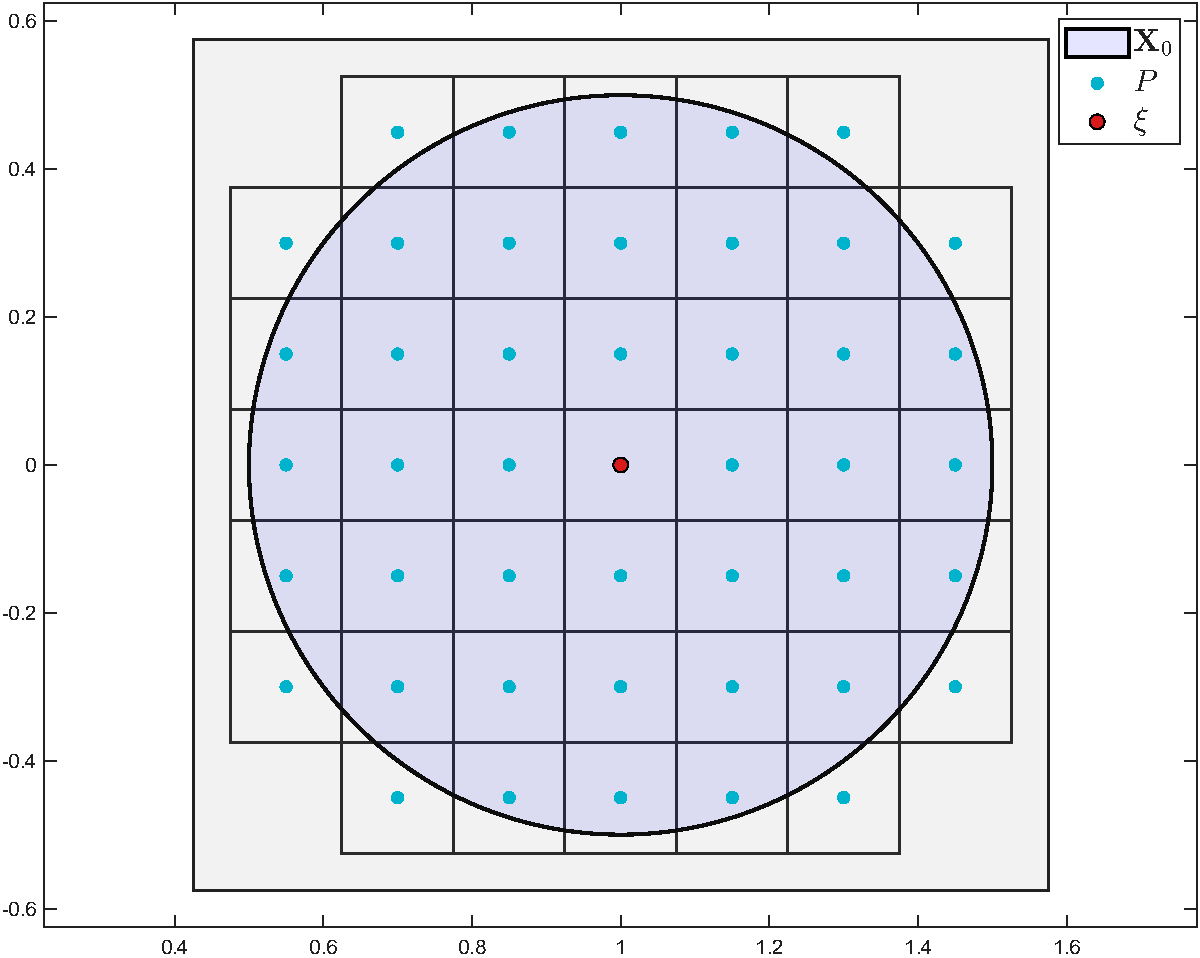
\includegraphics[scale=0.4]{fig/initial_grid.pdf}
    \caption{Grid sampling of $\mathbb{X}_0$. Points in $P$ (light blue) are sampled around the center $\boldsymbol{\xi}$, and the union of $n$-cubes over-approximates $\mathbb{X}_0$.}
    \label{fig:initial_grid}
\end{figure}

\subsection{Control approach} 

For a fixed $j \in \{1, \dots, N\}$ and $\boldsymbol{\eta}_j \in P$, consider an alternative trajectory $\hat{\mathbf{x}}_{\boldsymbol{\eta}_j, \hat{\boldsymbol{\nu}}_j}(t)$ with initial condition $\hat{\mathbf{x}}_{\boldsymbol{\eta}_j, \hat{\boldsymbol{\nu}}_j}(0) = \boldsymbol{\eta}_j$ and input $\hat{\boldsymbol{\nu}}_j(t)$. The nominal trajectory is $\mathbf{x}_{\boldsymbol{\xi}, \boldsymbol{\nu}}(t)$ with $\mathbf{x}_{\boldsymbol{\xi}, \boldsymbol{\nu}}(0) = \boldsymbol{\xi}$ and input $\boldsymbol{\nu}(t)$. To satisfy \eqref{def:contraction} for this pair of $\boldsymbol{\xi}$ and $\boldsymbol{\eta}_j$ we must find corresponding nominal and alternative controllers $\boldsymbol{\nu}$ and $\hat{\boldsymbol{\nu}}_j$, respectively. We define the state error $\mathbf{e}_j = \mathbf{x} - \hat{\mathbf{x}}_j$, with $\mathbf{e}_j(0) = \boldsymbol{\xi} - \boldsymbol{\eta}_j$.
\begin{lemma}\label{lemma:khalil}
\cite{khalil2002} Let $V:\mathbb{R}^n \to \mathbb{R}_{\ge 0}$ be a positive definite function of the error. Suppose there exist controllers $\boldsymbol{\nu}$ and $\hat{\boldsymbol{\nu}}_j$, such that along the error dynamics, it holds that $\dot V(\mathbf{e}_j) \le -\alpha(V(\mathbf{e}_j))$, for all $t \in \mathbb{R}_{\ge 0}$, where $\alpha$ is a locally Lipschitz class-$\mathcal{K}$ function. Then, there exists a class-$\mathcal{K} \mathcal{L}$ function $\zeta$ such that $\|\mathbf{e}_j(t)\| \le \zeta(\|\mathbf{e}_j(0)\|,t)$ for all $j = 1, \dots, N$ and $t \in \mathbb{R}_{\ge 0}$.
\end{lemma}
Namely, if the controllers $\boldsymbol{\nu}$ and $\hat{\boldsymbol{\nu}}_j$ satisfy the Lyapunov inequality $\dot V(\mathbf{e}_j) \le -\alpha(V(\mathbf{e}_j))$, then \eqref{eq:contraction} holds for the trajectory pair $(\mathbf{x}_{\boldsymbol{\xi},\boldsymbol{\nu}}, \hat{\mathbf{x}}_{\boldsymbol{\eta}_j,\hat{\boldsymbol{\nu}}_j})$. Define the augmented state and input $\bar{\mathbf{x}}_j = (\mathbf{x}, \hat{\mathbf{x}}_j)$ and $\bar{\mathbf{u}}_j = (\mathbf{u}, \hat{\mathbf{u}}_j)$. Using the system dynamics in \eqref{eq:system}, the derivative of $V(\mathbf{e}_j)$ can be written as an affine function of $\bar{\mathbf{u}}_j$. Consequently, the Lyapunov inequality can be expressed as
\begin{equation} \label{eq:lyapunov_ineq}
    -\left[ L_{\bar{\mathbf{f}}} V (\bar{\mathbf{x}}_j) + \alpha(V(\bar{\mathbf{x}}_j)) \right] - L_{\bar{\mathbf{g}}} V (\bar{\mathbf{x}}_j) \, \bar{\mathbf{u}}_j \ge \mathbf{0},  
\end{equation}
with $\bar{\mathbf{f}}$, $\bar{\mathbf{g}}$ defined in \eqref{eq:augmented_system}.

Writing \eqref{eq:lyapunov_ineq} for all pairs $(\mathbf{x}_{\boldsymbol{\xi},\boldsymbol{\nu}}, \hat{\mathbf{x}}_{\boldsymbol{\eta}_j,\hat{\boldsymbol{\nu}}_j})$, $j = 1, \dots, N$, yields a set of $N$ inequalities whose simultaneous satisfaction can be verified by solving
\begin{equation} \label{eq:qp2}
    \begin{aligned}
        c(\bar{\mathbf{x}}) = \max_{t, \bar{\mathbf{u}}} \quad & t \\[-5pt]
        \text{s.t.} \quad & \mathbf{q}_1(\bar{\mathbf{x}}) + \mathbf{Q}_2(\bar{\mathbf{x}}) \, \bar{\mathbf{u}}
        \ge t \mathbf{1}, \\
        & \bar{\mathbf{u}} \in \mathbb{U}^{N+ 1},
    \end{aligned}
\end{equation}
where $\bar{\mathbf{x}} = (\mathbf{x, \hat{\mathbf{x}}_1}, \dots, \hat{\mathbf{x}}_N)$ and $\bar{\mathbf{u}} = (\mathbf{u, \hat{\mathbf{u}}_1}, \dots, \hat{\mathbf{u}}_N)$, and
\[
    \mathbf{q}_1(\bar{\mathbf{x}}) = \begin{bmatrix} 
    -L_{\bar{\mathbf{f}}} V (\bar{\mathbf{x}}_1) - \alpha(V(\bar{\mathbf{x}}_1)) \\ \vdots \\ -L_{\bar{\mathbf{f}}} V (\bar{\mathbf{x}}_N) - \alpha(V(\bar{\mathbf{x}}_N)) 
    \end{bmatrix},
\]
\begin{equation*}
    \begin{aligned}
        &\mathbf{Q}_2(\bar{\mathbf{x}}) = \\[3pt]
        &\begin{bmatrix} 
        -L_{\mathbf{g}} V (\mathbf{x}) & \! \! \! -L_{\mathbf{g}} V (\hat{\mathbf{x}}_1) & \! \! \! \mathbf{0}^\top & \! \! \! \dots & \! \! \! \mathbf{0}^\top \\ 
        -L_{\mathbf{g}} V (\mathbf{x}) & \! \! \! \mathbf{0}^\top & \! \! \! -L_{\mathbf{g}} V (\hat{\mathbf{x}}_2) & \! \! \! \dots & \! \! \! \mathbf{0}^\top \\ \vdots & \! \! \! \vdots & \! \! \! \ddots & \! \! \! \ddots & \! \! \! \vdots \\ -L_{\mathbf{g}} V (\mathbf{x}) & \! \! \! \mathbf{0}^\top & \! \! \! \dots & \! \! \! \dots & \! \! \! -L_{\mathbf{g}} V (\hat{\mathbf{x}}_N)
        \end{bmatrix}.
    \end{aligned}
\end{equation*}
If $\mathbb{U}$ is polytopic, \eqref{eq:qp2} is a linear program. The optimal value $c(\bar{\mathbf{x}})$ represents the largest robustness margin with respect to violation of the $N$ Lyapunov inequalities at $\bar{\mathbf{x}}$.

Since $\mathbf{f}$, $\mathbf{g}$ and $\alpha$ are locally Lipschitz, and $V$ is continuously differentiable, $\mathbf{q}_1$ and $\mathbf{Q}_2$ are locally Lipschitz in $\bar{\mathbf{x}}$. For a fixed $j \in \{1, \dots, N\}$ and fixed $\mathbf{x}$, $\hat{\mathbf{x}}_i$, for all $i \neq j$, we study how the $j^\text{th}$ inequality changes when $\hat{\mathbf{x}}_j$ varies within $B(\hat{\mathbf{x}}_j, r)$. Note that the $j^\text{th}$ inequality depends only on $\hat{\mathbf{x}}_j$ and the inputs $\bar{\mathbf{u}}_j = (\mathbf{u}, \hat{\mathbf{u}}_j)$. Suppose $q_1^j(\bar{\mathbf{x}}_j) = -L_{\bar{\mathbf{f}}} V (\bar{\mathbf{x}}_j) - \alpha(V(\bar{\mathbf{x}}_j))$ and $\mathbf{q}_2^j(\bar{\mathbf{x}}_j) = -\big( L_{\bar{\mathbf{g}}} V (\bar{\mathbf{x}}_j) \big)^\top$ are Lipschitz in $\hat{\mathbf{x}}_j$ on a compact set containing $B(\hat{\mathbf{x}}_j, r)$. Then there exist constants $L_{j, 1}$, $L_{j, 2} \ge 0$ such that for all $\hat{\mathbf{x}}_j,\hat{\mathbf{x}}_j' \in B(\hat{\mathbf{x}}_j, r)$
\[
    |q_1^j(\bar{\mathbf{x}}_j) - q_1^j(\bar{\mathbf{x}}_j')| \le L_{j,1} \|\hat{\mathbf{x}}_j - \hat{\mathbf{x}}_j'\|_\infty,
\]
\[
    ||\mathbf{q}_2^j(\bar{\mathbf{x}}_j) - \mathbf{q}_2^j(\bar{\mathbf{x}}_j')||_\infty \le L_{j,2} \|\hat{\mathbf{x}}_j - \hat{\mathbf{x}}_j'\|_\infty,
\]
Thus, if $c(\bar{\mathbf{x}}) > 0$, Lipschitz continuity guarantees the existence of a neighborhood of $\bar{\mathbf{x}}$ in which $\hat{\mathbf{x}}_j$ may vary while $q_1^j(\bar{\mathbf{x}}_j) + \big( \mathbf{q}_2^j(\bar{\mathbf{x}}_j) \big)^\top \bar{\mathbf{u}}_j \le 0$ remains satisfied. 

\begin{proposition}
    Let $(c(\bar{\mathbf{x}}), \bar{\mathbf{u}}^\star(\bar{\mathbf{x}}))$ be the optimal solution of \eqref{eq:qp2} at $\bar{\mathbf{x}}$. For a fixed $j \in \{1,\dots,N\}$ and fixed $\mathbf{x}$, $\hat{\mathbf{x}}_i$, for all $i \neq j$,  define $\bar{\mathbf{u}}_j^\star = (\mathbf{u}^\star, \hat{\mathbf{u}}_j^\star)$, i.e., the components of $\bar{\mathbf{u}}^\star$ that appear in the $j^\text{th}$ inequality, and
    \[
        \rho_j := \frac{2 \, c(\bar{\mathbf{x}})} {L_{j,1}+L_{j,2}\|\bar{\mathbf{u}}_j^\star\|_\infty}.
    \]
    If $\rho_j \ge r$, for any $\bar{\mathbf{x}}' = (\mathbf{x}, \hat{\mathbf{x}}_1, \dots, \mathbf{x}_{j-1}, \hat{\mathbf{x}}_j', \mathbf{x}_{j+1}, \dots, \hat{\mathbf{x}}_N)$ with $\hat{\mathbf{x}}_j' \in B(\hat{\mathbf{x}}_j,r)$, the $j^\text{th}$ inequality remains satisfied, i.e., $q_1^j(\bar{\mathbf{x}}_j) + \big( \mathbf{q}_2^j(\bar{\mathbf{x}}_j) \big)^\top \bar{\mathbf{u}}_j^\star \ge 0$.
\end{proposition}

\begin{proof}
From \eqref{eq:qp2}, we get $q_1^j(\bar{\mathbf{x}}_j) + \big( \mathbf{q}_2^j(\bar{\mathbf{x}}_j) \big)^\top \bar{\mathbf{u}}_j^\star \ge c(\bar{\mathbf{x}}) \mathbf{1}$. For any $\bar{\mathbf{x}}' = (\mathbf{x}, \hat{\mathbf{x}}_1, \dots, \mathbf{x}_{j-1}, \hat{\mathbf{x}}_j', \mathbf{x}_{j+1}, \dots, \hat{\mathbf{x}}_N)$ with $\hat{\mathbf{x}}_j' \in B(\hat{\mathbf{x}}_j,r)$,
\[
    q_1^j(\bar{\mathbf{x}}_j') + \big( \mathbf{q}_2^j(\bar{\mathbf{x}}_j') \big)^\top \bar{\mathbf{u}}^\star
\]
\begin{equation} \label{eq:x'}
    \ge \big( q_1^j(\bar{\mathbf{x}}_j') - q_1^j(\bar{\mathbf{x}}_j) \big) + \big( \mathbf{q}_2^j(\bar{\mathbf{x}}_j') - \mathbf{q}_2^j(\bar{\mathbf{x}}_j) \big)^\top \bar{\mathbf{u}}_j^\star +  c(\bar{\mathbf{x}}).
\end{equation}
Since $\|\hat{\mathbf{x}}_j - \hat{\mathbf{x}}_j'\|_\infty \le \tfrac{r}{2}$ for any $\hat{\mathbf{x}}_j$, $\hat{\mathbf{x}}_j' \in B(\hat{\mathbf{x}}_j, r)$, we have
\[
    || \big( q_1^j(\bar{\mathbf{x}}_j') - q_1^j(\bar{\mathbf{x}}_j) \big) + \big( \mathbf{q}_2^j(\bar{\mathbf{x}}_j') - \mathbf{q}_2^j(\bar{\mathbf{x}}_j) \big)^\top \bar{\mathbf{u}}_j^\star ||_\infty
\] \[
    \leq || q_1^j(\bar{\mathbf{x}}_j') - q_1^j(\bar{\mathbf{x}}_j) ||_\infty + || \mathbf{q}_2^j(\bar{\mathbf{x}}_j') - \mathbf{q}_2^j(\bar{\mathbf{x}}_j) ||_\infty \,||\bar{\mathbf{u}}_j^\star ||_\infty
\] \[
    \leq L_{j, 1} \|\hat{\mathbf{x}}_j - \hat{\mathbf{x}}_j'\|_\infty + L_{j, 2} \|\hat{\mathbf{x}}_j - \hat{\mathbf{x}}_j'\|_\infty  \,||\bar{\mathbf{u}}_j^\star ||_\infty
\] 
\begin{equation} \label{eq:x'2}
    \leq (L_{j, 1} + L_{j, 2} \,||\bar{\mathbf{u}}^\star ||_\infty) \, \frac{r}{2} \leq (L_{j, 1} + L_{j, 2} \,||\bar{\mathbf{u}}_j^\star ||_\infty) \, \frac{\rho_j}{2} \leq c(\bar{\mathbf{x}}),
\end{equation}
if $\rho_j \ge r$. From \eqref{eq:x'} and \eqref{eq:x'2}, $q_1^j(\bar{\mathbf{x}}_j) + \big( \mathbf{q}_2^j(\bar{\mathbf{x}}_j) \big)^\top \bar{\mathbf{u}}_j^\star \ge 0$, which completes the proof.
\end{proof}

%%%%%%%%%%%%%%%%%%%%%%%%%%%%%%%%%%%%%%%%%%%%%%%%%%%%%%%%%%%%%%%%%%%%%%%%%%%%%%%%
\section{Case Study}

In this section, we demonstrate the proposed framework on a robot operating in a 2D workspace. The objective is to simultaneously enforce a reach-avoid specification and $\delta$-approximate infinite-horizon opacity using the CBF-based QP developed in Section~\ref{subsec:qp}.

We consider a single-integrator
\begin{equation}
    \dot{\mathbf{x}} = \mathbf{u}, \quad \mathbf{u} = \{ \mathbf{u} \in \mathbb{U} \mid -2 \leq u_i \leq 2\},
\end{equation}
with state $\mathbf{x} = (x_1, x_2)^\top$ and input $\mathbf{u} = (u_1, u_2)^\top \in \mathbb{R}^2$. The trajectories start from the initial set, i.e., $\mathbf{x}(0) = \mathbf{x}_0 \in \mathbb{X}_0$. The system output is given by $\mathbf{y} = \mathbf{h}(\mathbf{x}) = \mathbf{x}$, i.e., the intruder observes the position directly, up to precision $\delta$.

The workspace contains two unsafe regions (obstacles) $\mathbb{X}_u^{(1)}$ and $\mathbb{X}_u^{(2)}$, modeled as ellipsoids (cf. \eqref{eq:ellipsoid}) with centers $\mathbf{c}_u^{(1)} = (1, 1.5)^\top$, $\mathbf{c}_u^{(2)} = (3.4, 4.6)^\top$, and matrices $\mathbf{Q}_u^{(1)} = \operatorname{diag}(4, 1)$, $\mathbf{Q}_u^{(2)} = \operatorname{diag}(4, 4)$. Similarly, the three secret regions are described by
\begin{equation*}
    \begin{aligned}
        &\mathbf{c}_s^{(1)} = (5.5, 3.9)^\top, \, \mathbf{c}_s^{(2)} = (1.8, 3.5)^\top, \, \mathbf{c}_s^{(3)} = (4, 6.2)^\top, \\
        &\mathbf{Q}_s^{(1)} = \operatorname{diag}(\tfrac{4}{9}, \, \tfrac{4}{9}), \mathbf{Q}_s^{(2)} = \operatorname{diag}(1, 1), \, \mathbf{Q}_s^{(3)} = \operatorname{diag}(1, 1)
    \end{aligned}
\end{equation*}
Finally, for the goal region $\mathbb{X}_g$, we have
\begin{equation*}
    \mathbf{c}_g = (5.2, 7.1)^\top \text{ and } \mathbf{Q}_g = \operatorname{diag}(100, 100).
\end{equation*}

The objective is twofold: (i) the trajectory must reach the goal region $\mathbb{X}_g$ while avoiding unsafe regions $\mathbb{X}_u^{(1)}$, $\mathbb{X}_u^{(2)}$, and (ii) the trajectory must be $\delta$-approximate infinite-horizon opaque with respect to the secret set $\mathbb{X}_s = \bigcup_{i=1}^{3} \mathbb{X}_s^{(i)}$.

We set $\delta = 0.2$, that represents the measurement precision of the intruder. Thus, whenever the real trajectory enters any of the secret regions, there must exist an alternative trajectory whose output remains within distance $\delta$ of the real output, while remaining outside the secret set at the same time.

Opacity is enforced in the augmented state space using two CBFs. The first one enforces $\delta$-indistinghuisability (cf. \eqref{eq:delta_cbf}) and the second one guarantees that either the real or the alternative trajectory is always outside of any secret region (\eqref{eq:cbf_multiple_secret}). Safety with respect to the two obstacles is enforced via CBFs, one for each obstacle.

The QP as in \eqref{eq:qp} is solved online in sampled-data fashion. Starting from initial condition $\mathbf{x}_0 = (0, 0)^\top$ and $\hat{\mathbf{x}}_0 = (0, 0.1)^\top$ for the real and the alternative trajectory, respectively, the optimization-based controller drives the system toward the goal region while satisfying safety and opacity along the path. The resulting trajectories are presented in Fig.~\ref{fig:traj}. 
\begin{figure}[tb]
    \centering
    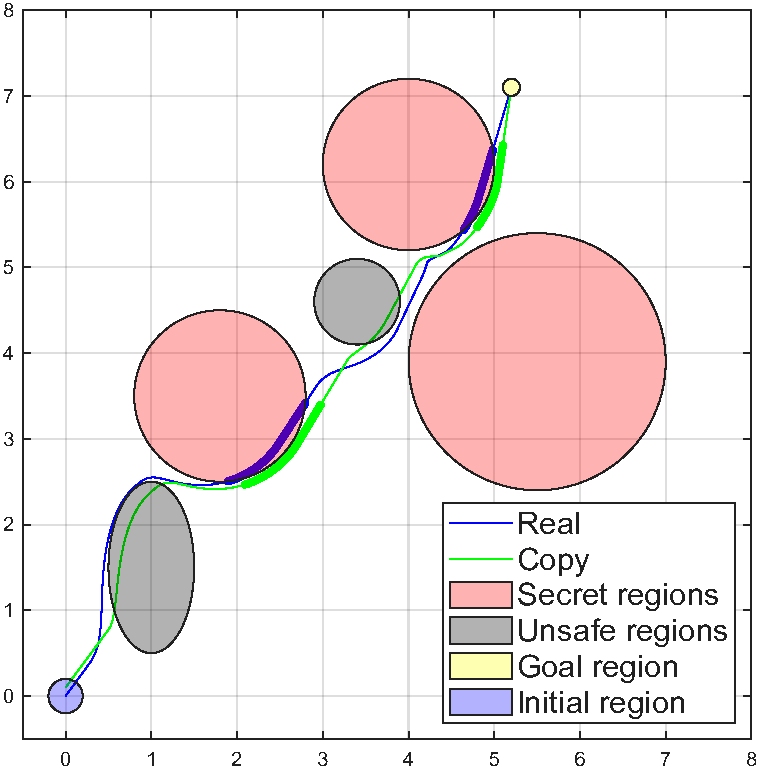
\includegraphics[scale=0.5]{fig/si0.2traj.pdf}
    \caption{Real and alternative trajectories for $\delta=0.2$}
    \label{fig:traj}
\end{figure}

This case study illustrates that the proposed CBF-based framework can simultaneously enforce reach-avoid specifications and continuous-time opacity constraints in a unified QP formulation.

% \begin{figure}[tb]
%     \centering
%     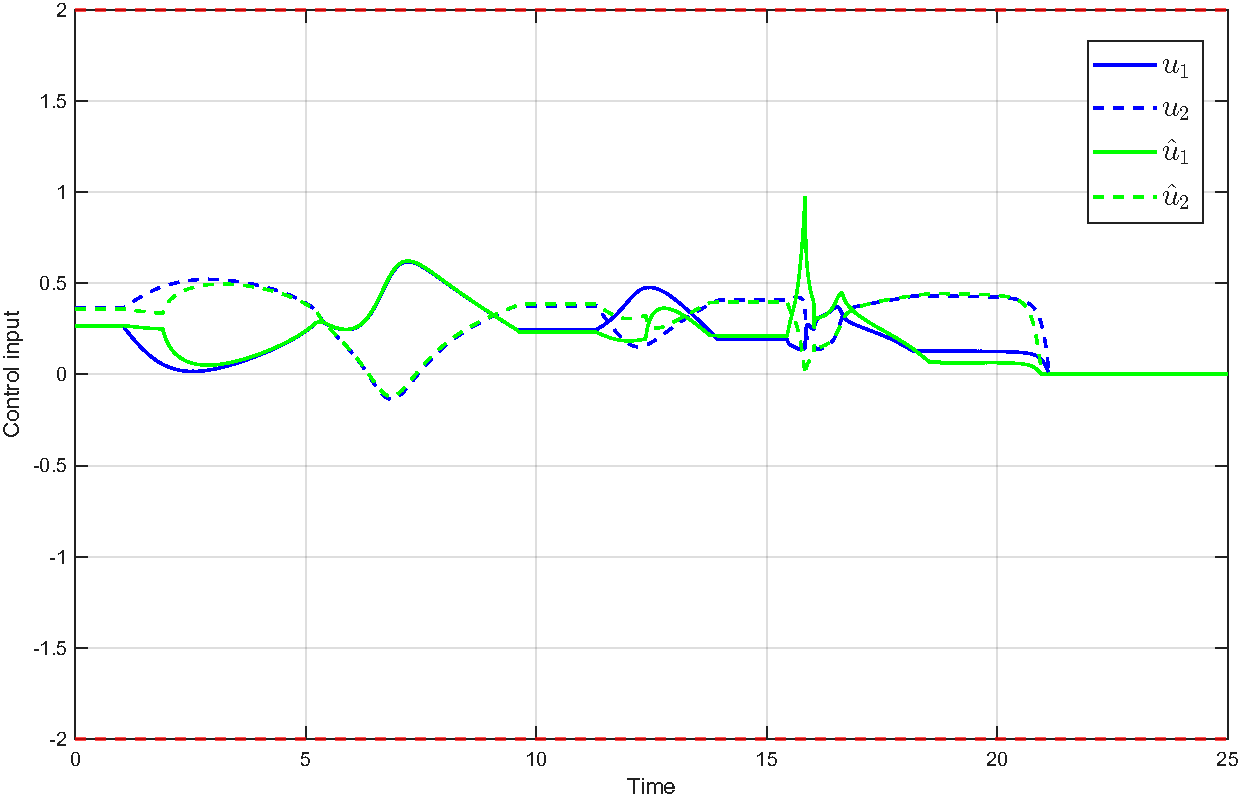
\includegraphics[scale=0.3]{fig/si0.2ctrl.pdf}
%     \caption{Control input}
%     \label{fig:ctrl}
% \end{figure}

% \begin{figure}[tb]
%     \centering
%     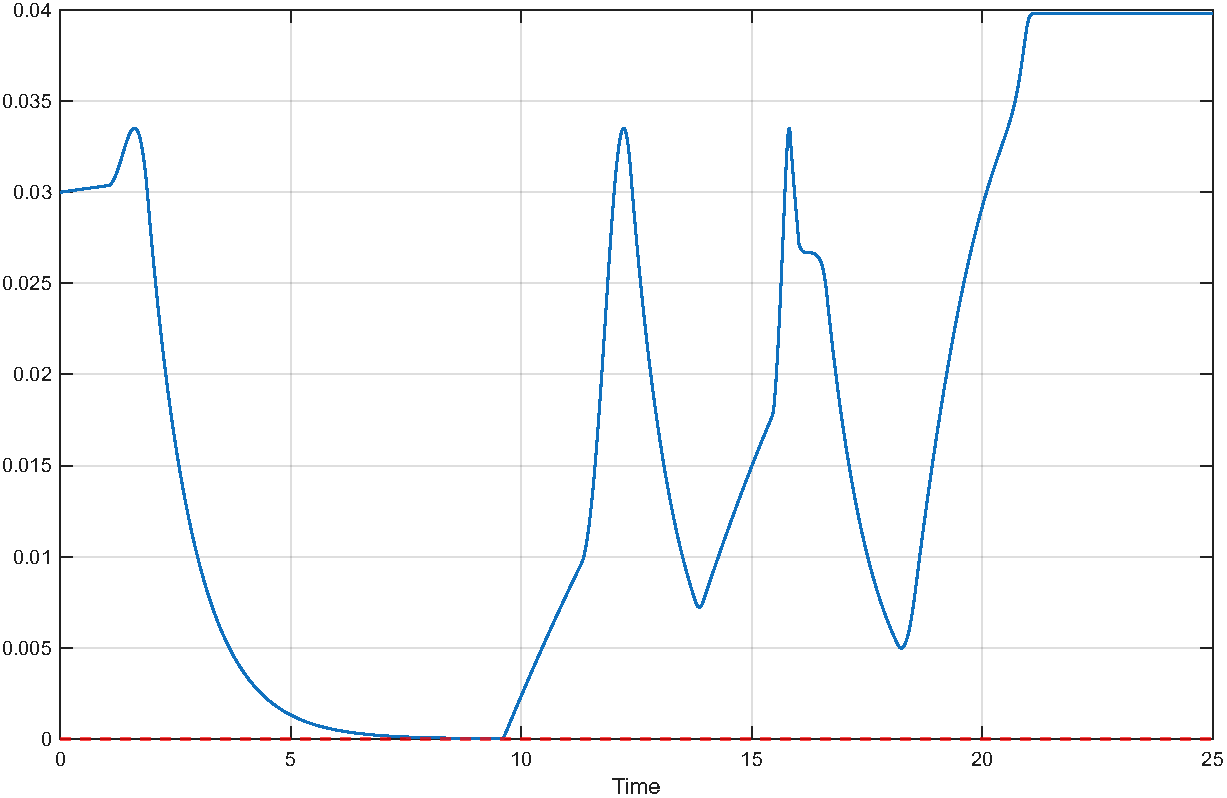
\includegraphics[scale=0.3]{fig/si0.2delta.pdf}
%     \caption{Indistinghuisability CBFs}
%     \label{fig:delta}
% \end{figure}

% \begin{figure}[tb]
%     \centering
%     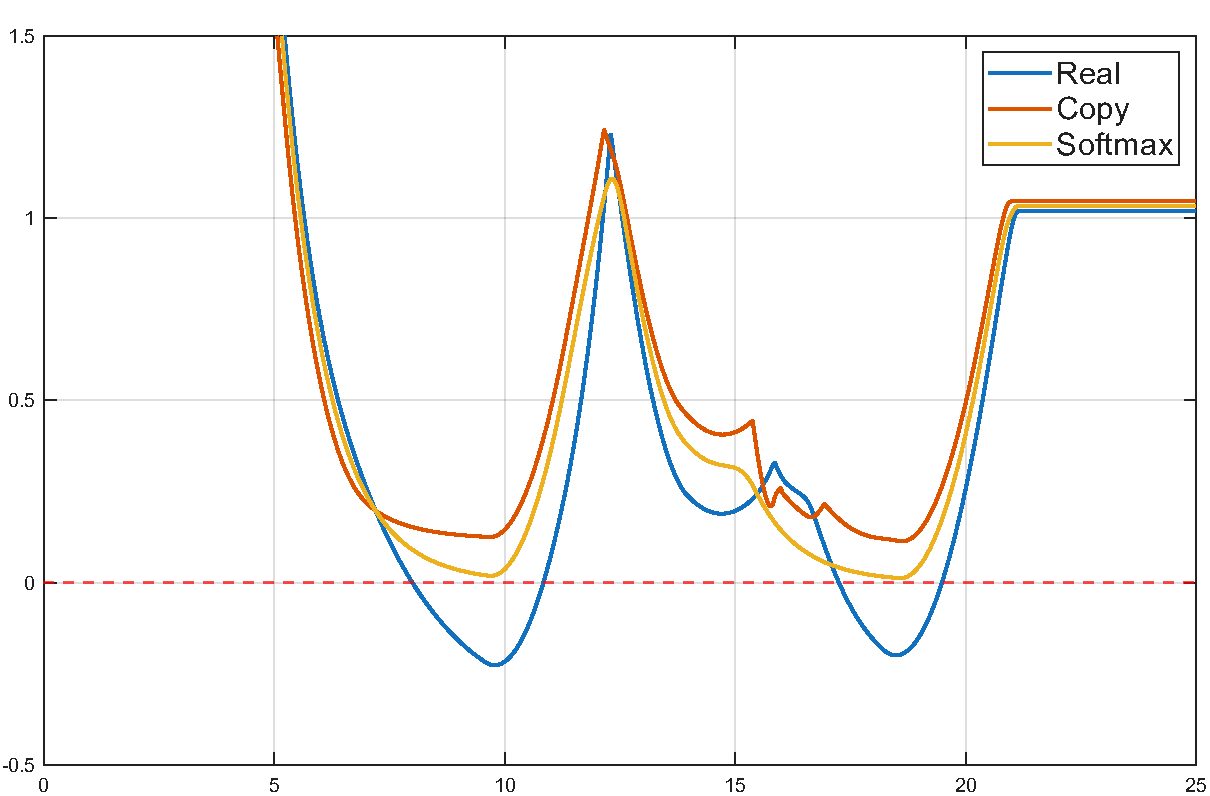
\includegraphics[scale=0.3]{fig/si0.2secret.pdf}
%     \caption{Secrecy CBFs}
%     \label{fig:secret}
% \end{figure}

% \begin{figure}[tb]
%     \centering
%     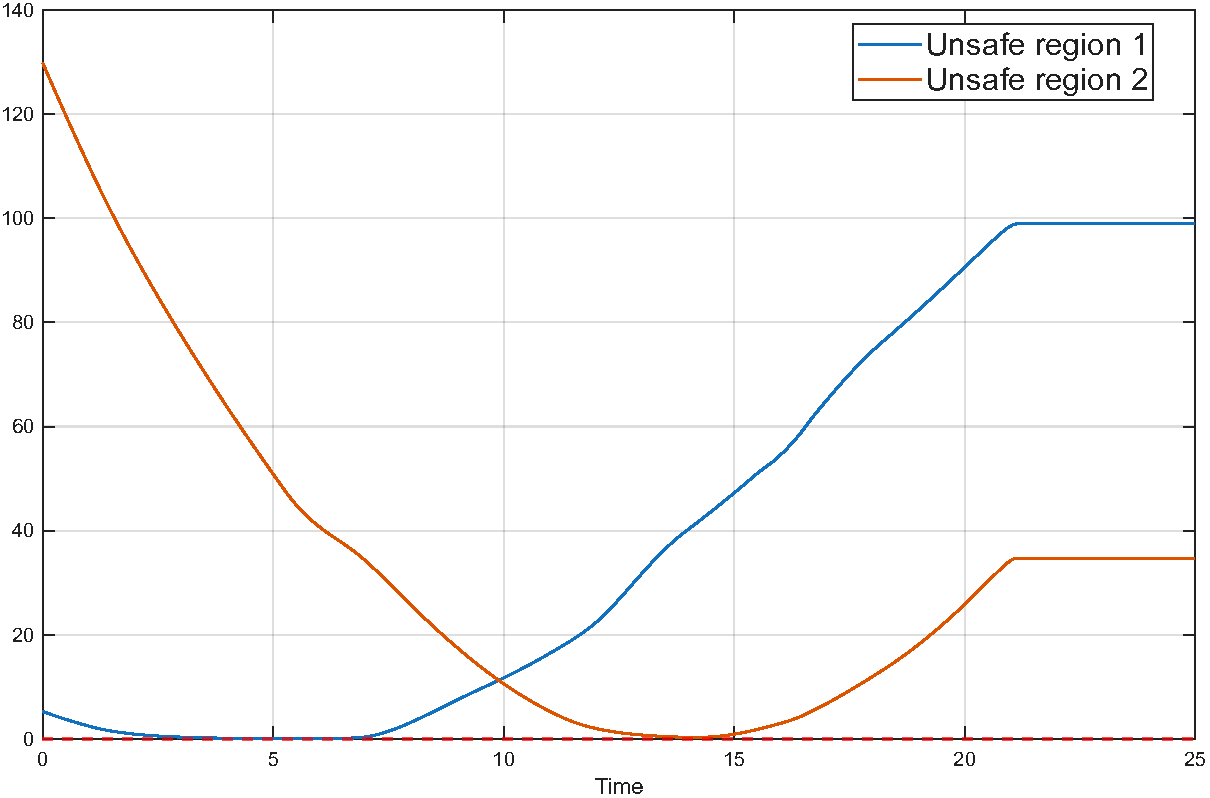
\includegraphics[scale=0.3]{fig/si0.2safety.pdf}
%     \caption{Safety CBFs}
%     \label{fig:safety}
% \end{figure}


%%%%%%%%%%%%%%%%%%%%%%%%%%%%%%%%%%%%%%%%%%%%%%%%%%%%%%%%%%%%%%%%%%%%%%%%%%%%%%%%
\section{Conclusion}

\addtolength{\textheight}{-12cm}   % This command serves to balance the column lengths on the last page of the document manually. It shortens the textheight of the last page by a suitable amount. This command does not take effect until the next page so it should come on the page before the last. Make sure that you do not shorten the textheight too much.


%%%%%%%%%%%%%%%%%%%%%%%%%%%%%%%%%%%%%%%%%%%%%%%%%%%%%%%%%%%%%%%%%%%%%%%%%%%%%%%%
\begin{thebibliography}{99}

% \bibitem{c2} W.-K. Chen, Linear Networks and Systems (Book style).	Belmont, CA: Wadsworth, 1993, pp. 123--135.

% \bibitem{c10} J. U. Duncombe, Infrared navigation Part I: An assessment of feasibility (Periodical style), IEEE Trans. Electron Devices, vol. ED-11, pp. 34--39, Jan. 1959.

% \bibitem{c13} S. P. Bingulac, On the compatibility of adaptive controllers (Published Conference Proceedings style), in Proc. 4th Annu. Allerton Conf. Circuits and Systems Theory, New York, 1994, pp. 8--16.

\bibitem{fainekos2009} G. E. Fainekos, A. Girard, H. Kress-Gazit, and G. J. Pappas, Temporal logic motion planning for dynamic robots, Automatica, vol. 45(2), pp. 343--352, 2009.

\bibitem{kloetzer2008} M. Kloetzer, and C. Belta, A fully automated framework for control of linear systems from temporal logic specifications, IEEE Trans. Autom. Control, vol. 53(1), pp. 287--297, 2008.

\bibitem{lavalle2006} S. M. LaValle, Planning algorithms. Cambridge Univ. Press, 2006.

\bibitem{karaman2011} S. Karaman, and E. Frazzoli, Sampling-based algorithms for optimal motion planning, Int. J. Robot. Res., vol. 30(7), pp. 846--894, 2011.

\bibitem{smith2011} S. L. Smith, J. Tumova, C. Belta, and D. Rus, Optimal path planning for surveillance with temporal-logic constraints, Int. J. Robot. Res., vol. 30(14), pp. 1695--1708, 2011.

\bibitem{wang2020} Y. Wang, S. Nalluri, and M. Pajic, Hyperproperties for robotics: planning via HyperLTL, in Proc. IEEE Int. Conf. Robot. Autom., 2020, pp. 8462--8468.

\bibitem{lafortune2018} S. Lafortune, F. Lin, and C. Hadjicostis, On the history of diagnosability and opacity in discrete event systems, Annu. Rev. Control, vol. 45, pp. 257--266, 2018.

\bibitem{clarkson2010} M. R. Clarkson, and F. B. Schneider, Hyperproperties, J. Comput. Secur., vol. 18(6), pp. 1157--1210, 2010.

\bibitem{clarkson2014} M. R. Clarkson, B. Finkbeiner, M. Koleini, K. K. Micinski, M. N. Rabe, and C. Sánchez, Temporal logics for hyperproperties, in Proc. Princ. Secur. Trust, 2014, pp. 265--284.

\bibitem{zhao2024} J. Zhao, S. Li, and X. Yin, A unified framework for verification of observational properties for partially-observed discrete-event systems, IEEE Trans. Autom. Control, vol. 69(7), pp. 4710--4717, 2024.

\bibitem{nguyen2017} L. V. Nguyen, J. Kapinski, X. Jin, L. V. Deshmukh, and T. T. Johnson, Hyperproperties of real-valued signals, in Proc. Proc. 15th ACM/IEEE Int. Conf. Formal Methods Models Syst. Des., 2017, pp. 104--113.

\bibitem{finkbeiner2015} B. Finkbeiner, M. N. Rabe, and C. Sánchez, Algorithms for Model Checking HyperLTL and HyperCTL$^*$, in Proc. 27th Int. Conf. Comput. Aided Verif. (CAV), 2015, pp. 30--48.

\bibitem{anand2024} M. Anand, V. Murali , A. Trivedi, and M. Zamani, Verification of hyperproperties for dynamical systems via barrier certificates, IEEE Trans. Autom. Control, vol. 69(10), pp. 6920--6934, 2024.

\bibitem{zhao2025} J. Zhao, B. Ye, X. Yu, R. Majumdar, X. Yin, Task and motion planning of dynamic systems using hyperproperties for signal temporal logics, arXiv preprint arXiv:2509.02184, 2025.

\bibitem{ames2014} A. D. Ames, J. W. Grizzle, and P. Tabuada, Control barrier function based quadratic programs with application to adaptive cruise control, in Proc. 53th IEEE Conf. Decis. Control, 2014, pp. 6271--6278.

\bibitem{ames2019} A. D. Ames, S. Coogan, M. Egerstedt, G. Notomista, K. Sreenath, and P. Tabuada, Control barrier functions: theory and applications, in Proc. 18th IEEE Eur. Conf. Control, 2019, pp. 3420--3431.

\bibitem{srinivasan2021} M. Srinivasan, and S. Coogan, Control of mobile robots using barrier functions under temporal logic specifications, IEEE Trans. Robot., vol. 37(2), pp. 363--374, 2021.

% \bibitem{srinivasan2018} M. Srinivasan, S. Coogan, and M. Egerstedt, Control of multi-agent systems with finite time control barrier certificates and temporal logic, in Proc. 57th IEEE Conf. Decis. Control, 2018, pp. 1991--1996.

\bibitem{lindemann2019} L. Lindemann, and D. V. Dimarogonas, Control barrier functions for
signal temporal logic tasks, IEEE Control Syst. Lett., vol. 3(1), pp. 96--101, 2019.

\bibitem{xu2015} X. Xu, P. Tabuada, J. W. Grizzle, and A. D. Ames, Robustness of control barrier functions for safety critical control, IFAC-PapersOnline, vol. 48(27), pp. 54--61. 2015.

\bibitem{kolathaya2019} S. Kolathaya, and A. D. Ames, Input-to-state safety with control barrier functions, IEEE Control Syst. Lett., vol. 3(1), pp. 108--113, 2019.

\bibitem{yang2023} S. Yang, and X. Yin, Secure your intention: On notions of pre-opacity in discrete-event systems, IEEE Trans. Autom. Control, vol. 68(8), pp. 4754--4766, 2023.

\bibitem{yin2021} X. Yin, M. Zamani, and S. Liu, On approximate opacity of cyber-physical systems, IEEE Trans. Autom. Control, vol. 66(4), pp. 1630--1645, 2021.

\bibitem{yu2022} X. Yu, X. Yin, S. Li, and Z. Li, Security-preserving multi-agent coordination for complex temporal logic tasks, Control Eng. Pract., vol. 123, 105130, 2022.

\bibitem{zhong2025} B. Zhong, S. Liu, M. Caccamo, and M. Zamani, Secure-by-construction synthesis for control systems, IEEE Trans. Autom. Control, vol. 70(6), pp. 4170--4177, 2025.

\bibitem{sontag1983} E. Sontag, A Lyapunov-like stabilization of asymptotic controllability, SIAM J. Control Opt., vol. 21(3), pp. 462--471, 1983.

\bibitem{artstein1983} E. Sontag, Stabilization with relaxed controls, Nonlinear Anal.: Theory, Methods Appl., vol. 7(11), pp. 1163--1173, 1983.

\bibitem{lohmiller1998} W. Lohmiller, and J.-J. E. Slotine, On contraction analysis for nonlinear systems, Automatica, vol. 34(6), pp. 683--696, 1998.

\bibitem{baier2008} C. Baier, and J. Katoen, Principles of model checking. MIT Press, 2008.

\bibitem{tan2022} X. Tan, and D. V. Dimarogonas, Compatibility checking of multiple control barrier functions for input constrained systems, in Proc. 61st IEEE Conf. Decis. Control, 2022, pp. 939--944.

\bibitem{khalil2002} H. K. Khalil, Nonlinear Systems. Prentice Hall, 2002.

\end{thebibliography}


\end{document}
